\RequirePackage{fix-cm}

\documentclass{birkjour}


\usepackage[T1]{fontenc}

\usepackage{graphicx}
\usepackage{svg}
\usepackage{amsfonts}
\usepackage{url}
\usepackage{ulem}
\usepackage{lipsum}
\usepackage{algorithm2e}
\usepackage{mathtools}
\usepackage{amssymb}
\usepackage[hidelinks]{hyperref}
%\usepackage{caption}
\usepackage{subcaption}
%\usepackage{environ} % for actually working environements declaration
\usepackage[framemethod=TikZ]{mdframed}

\captionsetup[subfloat]{labelfont=normalfont}
\RestyleAlgo{ruled}
\SetKwProg{Fn}{Function}{}{} 
\SetKwRepeat{Do}{do}{while}
\DontPrintSemicolon
\normalem % disable underlining in algorithm2e environement
\newcommand{\funct}[1]{\(\mathtt{#1}\)}

\newtheorem{theorem}{Theorem}
\newtheorem{definition}{Definition}
\newtheorem{remark}{Remark}
\newtheorem{proposition}{Proposition}
\newtheorem{example}{Example}

\surroundwithmdframed[linewidth=2pt, leftline=true, rightline=false, topline=false, bottomline=false, linecolor=black, innerleftmargin=10pt, innerrightmargin=10pt, innertopmargin=0pt, innerbottommargin=0pt]{proof}

\surroundwithmdframed[linewidth=1pt, leftline=true, rightline=true, topline=true, bottomline=true, linecolor=black, innerleftmargin=10pt, innerrightmargin=10pt, innertopmargin=10pt, innerbottommargin=10pt]{example}

\begin{document}


%\title{Using pencils to extract points from conic intersection objects in Geometric Algebra}
%\title{Using pencils to extract points from conic intersection in Geometric Algebra}
\title{Conics, their pencils and intersections in Geometric Algebra}
%\title{Extracting points from pencils of conics using Geometric Algebra}
% \title{Conics in Geometric Algebra: everthing is a pencil from which points can be extracted}
% \title{Exploring conic through Geometric Algebra: pencil and intersection points extraction}
% \title{Two conics intersect into a pencil, extracting points from a bad joke}

\author[Chomicki C.]{Cl\'ement Chomicki}
\address{LIGM, Universit\'e Gustave Eiffel, CNRS, France}
\email{clement.chomicki@univ-eiffel.fr}

\author[Breuils S.]{St\'ephane Breuils}
\address{LAMA, Universit\'e Savoie Mont-Blanc, CNRS, France}
\email{stephane.breuils@univ-smb.fr}

\author[Biri V.]{Venceslas Biri}
\address{LIGM, Universit\'e Gustave Eiffel, CNRS, France}
\email{venceslas.biri@univ-eiffel.fr}

\author[Nozick V.]{Vincent Nozick}
\address{LIGM, Universit\'e Gustave Eiffel, CNRS, France}
\email{vincent.nozick@univ-eiffel.fr}

\date{ }% The correct dates will be entered by the editor


\newcommand{\qcgaobject}[1]{\overset{\mbox{\tiny QC2GA}}{#1}}
\newcommand{\gacobject}[1]{\overset{\mbox{\tiny GAC}}{#1}}
\newcommand{\gavec}[3][e]{\({#1_{#2_{#3}}}\)}
% force a numbering (i) and increment the counter
% used in align environement or in similar cases
\newcommand{\forcenumbering}{(\refstepcounter{equation}\theequation)}

\begin{abstract}
%Conic sections find extensive applications across various disciplines like optics, physics, and numerous other fields such as 3D modeling. Consequently, the Geometric Algebra community is actively involved in developing frameworks aimed at efficiently supporting and manipulating conics. While algebras specialized in representing conics do recognize and support conic-conic intersection objects, an elegant formula for extracting intersection points from these objects was previously unavailable. 
This paper presents an approach for extracting points from conic intersections by using the concept of pencils. This method is based on QC2GA - the two-dimensional version of QCGA (Quadric Conformal Geometric Algebra) - that is demonstrated to be equivalent to GAC (Geometric Algebra for Conics). A new interpretation of QC2GA and its objects based on pencils of conics and point space elements is presented, enabling the creation, constraining, and exploitation of pencils of conics. A Geometric Algebra method for computing the discriminants and center point of a conic will also be presented, enabling the proposition of an algorithm for extracting points from a conic intersection object.
\end{abstract}
\keywords{Conics, Geometric Algebra, Projective Geometry, Clifford Algebra, Quadric Conformal Geometric Algebra (QCGA), Geometric Algebra for Conics (GAC), Pencil}


\maketitle


%%%%%%%%%%%%%%%%%%%%%%%%%%%%%%%%%%%%%%%%%%%%%%%%%%%%%%%%%%%%%%%%%%%%%%%%%%%%%%%%%%%%%%%%%%%%%%%%%%%%%%%%%%%%%
%%%%%%%%%%%%%%%%%%%%%%%%%%%%%%%%%%%%%%%%%%%%%%%%%%%%%%%%%%%%%%%%%%%%%%%%%%%%%%%%%%%%%%%%%%%%%%%%%%%%%%%%%%%%%
%%%%%%%%%%%%%%%%%%%%%%%%%%%%%%%%%%%%%%%%%%%%%%%%%%%%%%%%%%%%%%%%%%%%%%%%%%%%%%%%%%%%%%%%%%%%%%%%%%%%%%%%%%%%%
%%%%%%%%%%%%%%%%%%%%%%%%%%%%%%%%%%%%%%%%%%%%%%%%%%%%%%%%%%%%%%%%%%%%%%%%%%%%%%%%%%%%%%%%%%%%%%%%%%%%%%%%%%%%%
%%%%%%%%%%%%%%%%%%%%%%%%%%%%%%%%%%%%%%%%%%%%%%%%%%%%%%%%%%%%%%%%%%%%%%%%%%%%%%%%%%%%%%%%%%%%%%%%%%%%%%%%%%%%%

\section{Introduction} \label{sec:intro} Geometric Algebras (GA), commonly referred to as Clifford Algebras, constitute a robust and versatile mathematical framework, particularly well-suited for the study of geometry and related domains. GAs are often encountered in domains that intensively use matrix determinants, such as physics, and permit the expression of objects and operations with more elegance than what linear algebra allows. More advanced models can also be formulated with Geometric Algebras~\cite{gregory_elastic_2017,hestenes_zitterbewegung_1990,hestenes_new_2012}. GA can also be used to represent geometric primitives and their geometric transformations, which finds useful applications in computer graphics~\cite{de_keninck_non-parametric_2019}. Several propositions of GA-flavored neural networking have also been proposed~\cite{buchholz_optimal_2007,ruhe_geometric_2023}. For a comprehensive introduction to Geometric Algebras, the textbooks of Perwass and Dorst \cite{perwass_geometric_2009,dorst_geometric_2010} are recommended references. 

The inherent compatibility of Geometric Algebras with polynomial embedding~\cite{perwass_geometric_2009} facilitates a seamless integration of polynomial curves with Geometric Algebra, presenting a promising union. In light of this advantageous association, numerous Geometric Algebra frameworks have been devised to address the representation, transformation, and intersection of both curves and surfaces. For instance, one could cite CGA (Conformal Geometric Algebra)~\cite{dorst_geometric_2010}, which manipulates not only lines and planes but also spheres and circles.

Perwass~\cite{perwass_geometric_2009} initiated the exploration of representing conics constructed from five points using a blade-based approach within the algebra \(\mathbb{G}_{5,3}\). Although this algebra accommodates conic translations and rotations, it is introduced primarily as a proof of concept, intended for subsequent and more extensive development. Later on, Goldman et al. proposed \(\mathbb{R}(4,4)\)~\cite{goldman_r4_2015}, an algebraic structure comprising two projective \(\mathbb{R}^4\) bases capable of effectively supporting quadrics, including conics resulting from the removal of one dimension. Likewise, Easter et al. introduced DCGA (Double Conformal Geometric Algebra)~\cite{easter_double_2017}, which is composed of two CGA bases and allows the representation of general Darboux cyclides, thereby embedding quadrics. However, a common limitation observed in both of these algebras is the absence of curve and surface constructions based on control points, which is a popular feature in mainstream GAs.

Breuils et al. introduced QCGA (Quadric Conformal Geometric Algebra)~\cite{breuils2018quadric,breuils_three-dimensional_2019} as an extension of Perwass' Conformal Conic Algebra. QCGA not only explores intersections and transformations but also extends its capabilities to handle quadric surfaces in a 3D space. By reducing the dimensionality of QCGA by removing seven vectors from its basis, one obtains QC2GA, a specialized algebra specifically designed for the manipulation of conics in a 2D space. More recently, Hrdina et al. proposed GAC (Geometric Algebra for Conics)~\cite{hrdina_geometric_2018}, which is another extension of Perwass' algebra but fully dedicated to 2D and conics. Both of these algebras, akin to Perwass' approach, represent conics as blades of points (meaning that we can construct a conic from five of its points). However, a notable difference emerges between the two: QCGA includes a third spatial dimension, making QC2GA easier to extend in 3D, while GAC offers a more extensive repertoire of geometric transformations.

Despite their respective strengths, both QCGA and GAC share a common limitation, namely the absence of a mechanism to process conic intersection objects into points, as well as other highly desirable functionalities such as identifying the type (ellipse, parabola, hyperbola, \dots) and potential degeneracy of a conic. Furthermore, some degenerate conics are pairs of lines, and in such cases, the capability to extract these two lines would be useful. Neither QCGA nor GAC manage to extract interesting features like conic center and various pertinent lines. Even if Byrtus et al.~\cite{byrtus_specific_2021} proposed a method for extracting the intersection points of specific couples of conics, there is yet no method to compute the intersection of general conics.

This paper is an extension of~\cite{chomicki_intersection_2023}.
It formalizes its predecessor with new propositions, including a more robust definition of point-space elements and pencils of conics used as the basis of a complete reinterpretation of QC2GA. 
This new framework allows one to fully understand and manipulate every object as pencils of conics or Points-Space Elements and permits constraining, extending, or sampling objects from them.
%It has the ambition to augment its predecessor with a significant amount of new propositions, including a more robust definition of point-space elements and pencils of conics used as the basis of a complete reinterpretation of QC2GA. 
%This new framework allows to fully understand and manipulate every object as pencils of conics or Points-Space Elements and permits to constrain, extend, or sample objects from them. 
The new elements introduced are used to compute the discriminants and centers of conics, and numerical results are presented, attesting to the robustness of the proposed algorithm. The paper is organized as follows: Sec.~\ref{sec:notations} presents the notation employed in this paper. Sec.~\ref{sec:State_of_the_art} introduces conics and their pencils in their classical algebraic framework. Sec.~\ref{sec:QCGA_and_GAC} presents two Geometric Algebras for conics, QC2GA and GAC, and proves their equivalence. Next, Sec.~\ref{sec:points} introduces points and points-space elements in QC2GA, serving as a base for Sec.~\ref{sec:pencils}, which proposes a novel interpretation of QC2GA based on pencil of conics. Sec.~\ref{sec:discriminants} then describes a new way to compute the determinants of a conic, used in Sec.~\ref{sec:extraction} in our algorithm of point extraction from conics intersections in QC2GA, which is the core contribution of this paper. Finally, the numerical results of this algorithm are listed in Sec.~\ref{sec:experiments}.
%%%%%%%%%%%%%%%%%%%%%%%%%%%%%%%%%%%%%%%%%%%%%%%%%%%%%%%%%%%%%%%%%%%%%%%%%%%%%%%%%%%%%%%%%%%%%%%%%%%%%%%%%%%%%
\section{Notations}
\label{sec:notations}
When referring to Geometric Algebra, most of the notations in this paper are inspired from~\cite{dorst_geometric_2010} and~\cite{perwass_geometric_2009}. In addition, we specify the following notations:
\begin{equation*}
\def\arraystretch{1.7}
\setlength\arraycolsep{3ex}
\begin{array}{r|l}
    m_{i_1 \dots i_n}^{j_1 \dots j_m}(\mathrm{A}) &\parbox{\linewidth/2}{the minor of matrix A with rows \\
    \(j_1 \dots j_m\) and columns \(i_1 \dots i_n\) removed} \\
    A^c & \parbox{0.5\linewidth}{right complement~\cite{gunn2022bit} of multivector \(A\)} \\ 
    A^* & \parbox{0.5\linewidth}{dual~\cite{dorst_geometric_2010} of $A$ with \(A^*= A I^{-1}\)} \\
    \mbox{adj}(\mathrm{A}) & \parbox{0.5\linewidth}{classical adjoint / adjugate of matrix~\(\mathrm{A}\)} \\
    gr(A) & \mbox{grade of the blade \(A\)} \\
    \wedge\,, \vee & \mbox{wedge/outer (join) and antiwedge/anti-outer (meet) products} \\
    \overline{E} & \mbox{canonical algebraic basis of the vector space E~\cite{perwass_geometric_2009}}\\
    \mathrm{p}^n & \mbox{a tuple of \(n\) points} \\
    A \equiv B & \mbox{\(A\) equals \(B\) up to a non-zero scale}
\end{array}
\end{equation*}

%%%%%%%%%%%%%%%%%%%%%%%%%%%%%%%%%%%%%%%%%%%%%%%%%%%%%%%%%%%%%%%%%%%%%%%%%%%%%%%%%%%%%%%%%%%%%%%%%%%%%%%%%%%%%
%%%%%%%%%%%%%%%%%%%%%%%%%%%%%%%%%%%%%%%%%%%%%%%%%%%%%%%%%%%%%%%%%%%%%%%%%%%%%%%%%%%%%%%%%%%%%%%%%%%%%%%%%%%%%
\section{An overview of conics}
\label{sec:State_of_the_art}
This section gives a short introduction to conics as projective algebra objects.

\subsection{Conics representation}
\label{sec:conic-representation}
Evidence of conics dates back as far as 380 BC in ancient Greece, with the works of Menaechmus. Over the past couple of centuries, mathematicians have established connections between these planar curves and quadratic equations of two variables. They are nowadays common projective algebra objects.

Because conics have been studied for so long, various properties of conics are taken for granted by mathematicians, so the number of sources is not that high. Faucette's \cite{faucette_geometric_1996} reminds the reader that conics are affine planar polynomial curves of degree 2, which implies six parameters \(a,b,c,d,e,f\):
\begin{equation} \label{eq:conic_affine}
    C: ax^2 + by^2 + cxy + dx + ey + f = 0
\end{equation}
Some people tend to work in \(\mathbb{C}\) when having a purely algebraic approach, but this paper is about geometry, so the six parameters \(\left(a,b,c,d,e,f\right)\) are constrained to \(\mathbb{R}^6\).
Apart from a couple of specific degenerate cases, a conic can be interpreted as the intersection of an infinite cone with a plane, which is why they are often referred to as "\textit{conic sections}".
Because we follow a projective approach, a point of coordinates \(\left(x,y,w\right)^\top\) in \(\mathbb{P}^2\) turns any conics into a homogeneous polynomial of degree 2 of three variables:
\begin{equation} \label{eq:conic_projective}
    C: ax^2 + by^2 + cxy + dxw + eyw + fw^2 = 0
\end{equation}
This formulation supports finite points as well as points at infinity with \(w\) component equal to 0. Here, a conic \(C\) can be represented as an element of \(\mathbb{R}^6\), from its coefficient vector \(\left(a,b,c,d,e,f\right)^\top\).
A point \(\mathrm{p}\) of projective coordinates \(\left(x,y,w\right)^\top\) is an element of \(\mathbb{P}^2\). To evaluate a conic with a point, it is necessary to use the polynomial embedding \(Q: \mathbb{P}^2 \rightarrow \mathbb{R}^6\) with \(Q\big(\left(x,y,w\right)^\top\big) = \left(x^2,y^2,xy,xw,yw,w^2\right)^\top\).
The previous implicit Eq.~\eqref{eq:conic_projective} can then be found with a simple dot product:
\begin{equation} \label{eq:conic_R6}
        C \cdot Q(\mathrm{p}) = 0
\end{equation}
Another common representation of conics is based on their Hessian matrix \(\mathrm{H}_C\) and use points of the form \(\mathrm{p}=\left(x,y,w\right)^\top\).

\begin{align} \label{eq:conic_hessian}
    & \mathrm{p}\in C ~ \Leftrightarrow ~  \mathrm{p}^\top \mathrm{H}_C \mathrm{p} = 0 & \mbox{with~~}
    \mathrm{H}_C =  \def\arraystretch{1.2}\begin{bmatrix}
a && \frac{c}{2} && \frac{d}{2} \\
\frac{c}{2} && b &&\frac{e}{2} \\
\frac{d}{2} && \frac{e}{2} && f
\end{bmatrix}
\end{align}

The implicit representation of a conic presented so far is defined by six parameters \(a,b,c,d,e\) and \(f\). An alternative representation is built upon any five linearly independent points \(\mathrm{p}_1, \dots, \mathrm{p}_5\) lying on the conic. The conic can take a matrix form built from the \(\mathrm{p}_i\) and an additional point \(\mathrm{p} = (x,y,w)^\top\).
The Eq.~\eqref{eq:conic_projective} is then equivalent to the following vanishing determinant \cite{hartley_multiple_2004}:

\begin{align} \label{eq:PMat}
& \mathrm{p}\in C ~ \Leftrightarrow ~  \det\left(\mathrm{P}\right) = 0 &\mbox{with }\mathrm{P} = \begin{bmatrix} 
x^2 & y^2 & xy & xw & yw & w^2 \\
x_1^2 & y_1^2 & x_1y_1 & x_1w_1 & y_1w_1 & w_1^2 \\
x_2^2 & y_2^2 & x_2y_2 & x_2w_2 & y_2w_2 & w_2^2 \\
x_3^2 & y_3^2 & x_3y_3 & x_3w_3 & y_3w_3 & w_3^2 \\
x_4^2 & y_4^2 & x_4y_4 & x_4w_4 & y_4w_4 & w_4^2 \\
x_5^2 & y_5^2 & x_5y_5 & x_5w_5 & y_5w_5 & w_5^2
\end{bmatrix}
\end{align}
%This leads to an expression of the parameters \(a,b,c,d,e,f\) using the minors of \(\mathcal{\mathrm{p}}\):e
A conversion from the matrix form \(\mathrm{P}\) of Eq.~\eqref{eq:PMat} to the form \(a,b,c,d,e,f\) can be specified using the minors of \(\mathrm{P}\):
\begin{equation} \label{eq:minors}
\begin{aligned}
a &= \;\;\: m_1^1(\mathrm{P})& b &= -m_2^1(\mathrm{P}) & c &= \;\;\: m_3^1(\mathrm{P})  \\
d &= -m_4^1(\mathrm{P})& e &= \;\;\: m_5^1(\mathrm{P})  & f &= -m_6^1(\mathrm{P})
\end{aligned}
\end{equation}
This is equivalent to stating that \((a,b,c,d,e,f)\) forms the first row of the classical adjoint matrix of \(\mathrm{P}\).
There exists a generalization of this approach to any set of \(n\in[0,5]\) control points, which generates a \((5-n)\)-vector subspace of conics \cite{fulton_algebraic_1989}. 

%%%%%%%%%%%%%%%%%%%%%%%%%%%%%%%%%%%%%%%%%%%%%%%%%%%%%%%%%%%%%%%%%%%%%%%%%%%%%%%%%%%%%%%%%%%%%%%%%%%%%%%%%%%%%
\subsection{Type of conic and degenerate cases}
\label{sec:type_of_a_conic_and_degenerate}
As illustrated by Table~\ref{tab:det}, real-coefficiented conics can cover different kinds of geometry, ruled by two discriminants \(\Delta_2\) and \(\Delta_3\)~\cite{richter-gebert_perspectives_2011}:
%When \(\mathbb{K}=\mathbb{R}\), the type of the conic is ruled by these two discriminants \cite{Richter-Gerbert}: % ConicsAndTheirDuals
\begin{align} \label{eq:discriminants}
&\Delta_2(C) = m_{3}^3(\mathcal{H}_C) = ab - \frac{1}{4}c^2\\
&\Delta_3(C) = \det(\mathcal{H}_C) = abf + \frac{ced - c^2 f - bd^2 - ae^2 }{4}
\end{align}
\begin{table}[!ht]
\centering
\begin{tabular}{crl}
\(\Delta_2(C)\) & \(\Delta_3(C)\) & type of \(C\)\\
\hline
\(+\) & \(\ne 0\) & Ellipse (may be imaginary) \\
\(0\) & \(\ne 0\) & Parabola                   \\
\(-\) & \(\ne 0\) & Hyperbola                \\
\(+\) & \(0\)     & Point                    \\
\(0\) & \(0\)     & Two parallel lines       \\
\(-\) & \(0\)     & Two intersecting lines   \\
\end{tabular}
\caption{Shape of conic, ruled by their two determinants \(\Delta_2\) and \(\Delta_3\)}
\label{tab:det}
\end{table}
\begin{definition}[Degenerate conic]
A conic C is said degenerate (or reducible) iff. \(\Delta_3(C)=0\). A degenerate conic is either a pair of lines or a point.
\end{definition}
\begin{theorem}
A degenerate conic can be factored as a pair of complex lines.
\end{theorem}
\begin{proof}
Consider two complex lines \(l_1 = (u_1, v_1, w_1)^\top\) and \(l_2 = (u_2, v_2, w_2)^\top\). Each line corresponds to a polynomial \(u_1 x + v_1 y + w_1\) and \(u_2 x + v_2 y + w_2\), whose product results in the polynomial  \(u_1u_2x^2+v_1v_2 y^2+ xy(u_1v_2+u_2v_1)+(u_1w_2+u_2w_1)x+(v_1w_2+v_2w_1) y+ w_1w_2\) characterizing a conic \(C\) of parameters \((u_1u_2, v_1v_2, u_1v_2+u_2v_1,u_1w_2+u_2w_1,v_1w_2+v_2w_1, w_1w_2)\). As this yields \(\Delta_3(C) = 0\), a pair of complex lines is a degenerate conic.

Let \(C\) be a degenerate conic of hessian matrix \(\mathrm{H}_C\). The degeneracy implies that \(\det(\mathrm{H}_C)=0\) therefore there is a non-trivial solution \(l_1=(u_1,v_1,w_1)^\top\) so that \(\mathrm{H}_C l_1 =0\). Since the polynomial of the conic admits a root \(l_1\), it can be factorized into \(\left((x,y,w) l_1\right) \left((x,y,w) l_2\right)\) with \(l_2\) another line and for any point~\((x,y,w)^\top\).% Being a root of the polynomial of the conic, it can then be factored by it. 
Therefore, a degenerate conic \(C\) can always be factored into two complex lines \(l_1\) and \(l_2\).
%Its associated quadratic form is of grade less than 3. It is then factorable into two linear forms. 
\end{proof}

\begin{remark}
If a degenerate conic \(C\) is a pair of lines \(l_1 = (u_1, v_1, w_1)\) and \(l_2 = (u_2,v_2,w_2)\), then \(\displaystyle\Delta_2(C) = -\cfrac{\left(u_1v_2-u_2v_1\right)^2}{4} = -\frac{\|l_1\|^2\|l_2\|^2}{4}\sin^2(\widehat{l_1l_2})\).
\end{remark}

No matter how real or imaginary the coefficients of a conic are, if \(\Delta_3(C)=0\), the conic is said to be \textbf{degenerate} (or \textbf{reducible}). Degenerate conics can always be factored into two complex lines, which in the real case means that the conic is either a pair of real lines or a point (a pair of complex conjugate lines).


%%%%%%%%%%%%%%%%%%%%%%%%%%%%%%%%%%%%%%%%%%%%%%%%%%%%%%%%%%%%%%%%%%%%%%%%%%%%%%%%%%%%%%%%%%%%%%%%%%%%%%%%%%%%%
\subsection{Pencils}
This section presents objects known as pencils of conics. This concept, similar to those discussed in the literature such as Halsted's work from 1906~\cite{halsted_synthetic_1906}, is often mentioned but rarely clearly defined.
%This section introduces objects called pencils of conics, akin to what can be found in the literature~\cite{halsted_synthetic_1906} while also being rarely properly defined. 
In the context of this paper focusing on conics, pencils of conics will be called pencils.

\begin{definition}[Pencil]
%The vector space generated by conics is called a \textbf{pencil}. 
    \(n\) conics \(C_1,\dots,C_n\) form a vector space~\cite{halsted_synthetic_1906}, called \(n\)-pencil, or pencil of order \(n\).
    \begin{equation}
    \mathrm{Pencil}(C_1,\dots,C_n) = \left\{\sum_{i=1}^n\lambda_i Ci, ~~~~ \lambda_i \in \mathbb{R}\right\}
    \end{equation}
\end{definition}


\begin{proposition}
The intersection points of two conics \(C_a\) and \(C_b\) in \(\mathbb{R}^6\) are always equal to the intersection points of any two conics of their pencil 
\(\mathrm{Pencil}(C_a,C_b)\).
We can then refer to the intersection points of the conics of a pencil as the points of the pencil.
\end{proposition}
\begin{proof}
Consider two linearly independent conics \(C_a\) and \(C_b\). Consider a third linearly independent conic \(C_c\) in \(\mathrm{Pencil}(C_a,C_b)\). We have \(C_c = \lambda C_a + \mu C_b \) with \((\lambda,\mu) \in \left(\mathbb{R}^*\right)^2\).
Consider a point \(\mathrm{p}\) lying on the intersection of \(C_a\) and \(C_b\), meaning that \(C_a\cdot \mathrm{p} = 0\) and \(C_b\cdot \mathrm{p} = 0\).
It directly implies that  \(C_c \cdot \mathrm{p} = 0\) because of the bilinearity of the dot product. Hence, a point lying on the intersection of two conics also lies on any other conics of the pencil they generate.
Keep considering the same three conics \(C_a\), \(C_b\) and \(C_c\). \(C_c\in\mathrm{Pencil}(C_a,C_b)\) but it is also obvious that \(C_b\in\mathrm{Pencil}(C_a,C_c)\) and \(C_a\in\mathrm{Pencil}(C_b,C_c)\)  because \(C_a = \frac{-\mu C_b + C_c}{\lambda}\) and \(C_b = \frac{-\lambda C_a + C_c}{\mu}\). Hence \(C_a \cap C_b = C_a \cap C_b = C_a \cap C_c\), proving that every pair of conics in a pencil share the same intersection.
\end{proof}

This property is depicted in Fig.~\ref{fig:2-pencil}.

\begin{figure}[!ht]
    \begin{center}
    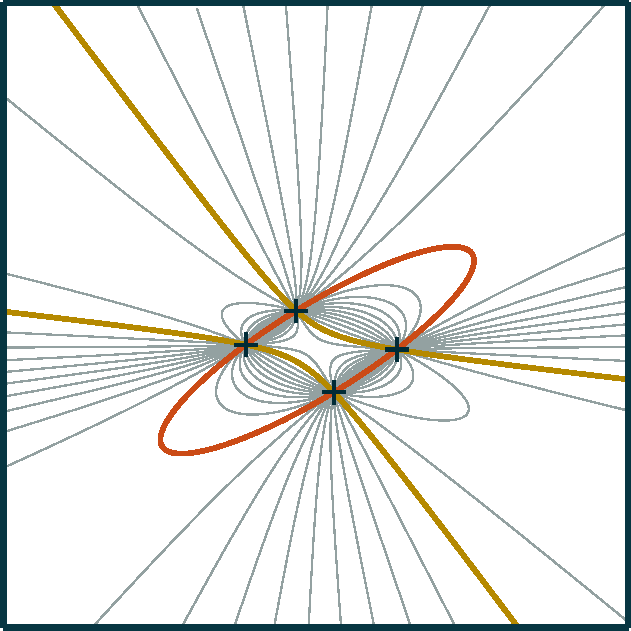
\includegraphics[width=0.49\linewidth]{4-inter-pencil}
    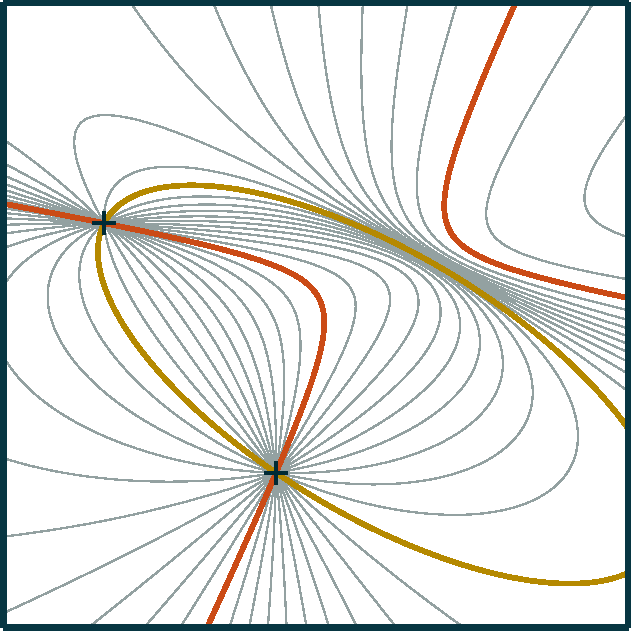
\includegraphics[width=0.49\linewidth]{2-inter-pencil}
    \end{center}
    \vspace{-8pt}
    \caption{A handful of conics (in grey) generated by the pencil built from two conics \(C_a\) and \(C_b\) (in red and yellow). \(C_a\) and \(C_b\) are of parameters \scriptsize
    \(\left(8.23237, 54.2227, 78.5338, 15.4803, 24.1495, 13.1695\right)\) \normalsize and
    \scriptsize\(\left(26.137, 60.0369, -68.5304, -15.8067, 27.4588, -3.48805\right)\)~\normalsize in the first image and
\scriptsize\(\left(286.036, 577.635, 5430.5, 1.14875, 283.959, -457.148\right)\) \normalsize and \scriptsize \(\left(-15.1326, 41.225, -80.2272, 39.5353, 8.24099, -2.03668\right)\) \normalsize in the second.}
    \label{fig:2-pencil}
\end{figure}

% Pour la 4-inter:
% Ca = [-0.0823237, -0.542227, -0.785338, -0.154803, -0.241495, -0.0131695]
% Cb = [0.26137, 0.600369, -0.685304, -0.158067, 0.274588, -0.0348805]
% Pour la 2-inter:
% Ca = [-0.286036, -0.577635, -0.54305, -0.00114875, -0.283959, 0.457148]
% Cb = [-0.151326, 0.41225, -0.802272, 0.395353, 0.0824099, -0.0203668]

% \begin{align}
% C_a &= (-0.0823237, -0.542227, -0.785338, -0.154803, -0.241495, -0.0131695) \\
% C_b &= (0.26137, 0.600369, -0.685304, -0.158067, 0.274588, -0.0348805) \\
% C_a &= (-0.286036, -0.577635, -0.54305, -0.00114875, -0.283959, 0.457148) \\
% C_b &= (-0.151326, 0.41225, -0.802272, 0.395353, 0.0824099, -0.0203668)
% \end{align}

%\(\left(-0.0823237, -0.542227, -0.785338, -0.154803, -0.241495, -0.0131695\right)\)
%\(\left(0.26137, 0.600369, -0.685304, -0.158067, 0.274588, -0.0348805\right)\)
% Pour la 2-inter:
% Ca = [-0.286036, -0.577635, -0.54305, -0.00114875, -0.283959, 0.457148]
% Cb = [-0.151326, 0.41225, -0.802272, 0.395353, 0.0824099, -0.0203668]


One could think that a \(2\)-pencil of conics is fully determined by its intersection points, but this only works for pencils having 4~intersection points.
For instance, Fig.~\ref{fig:3-pencil} shows three linearly independent conics sharing three intersection points, which implies that they cannot belong to the same 2-pencil.


\begin{figure}[!ht]
    \centering
%    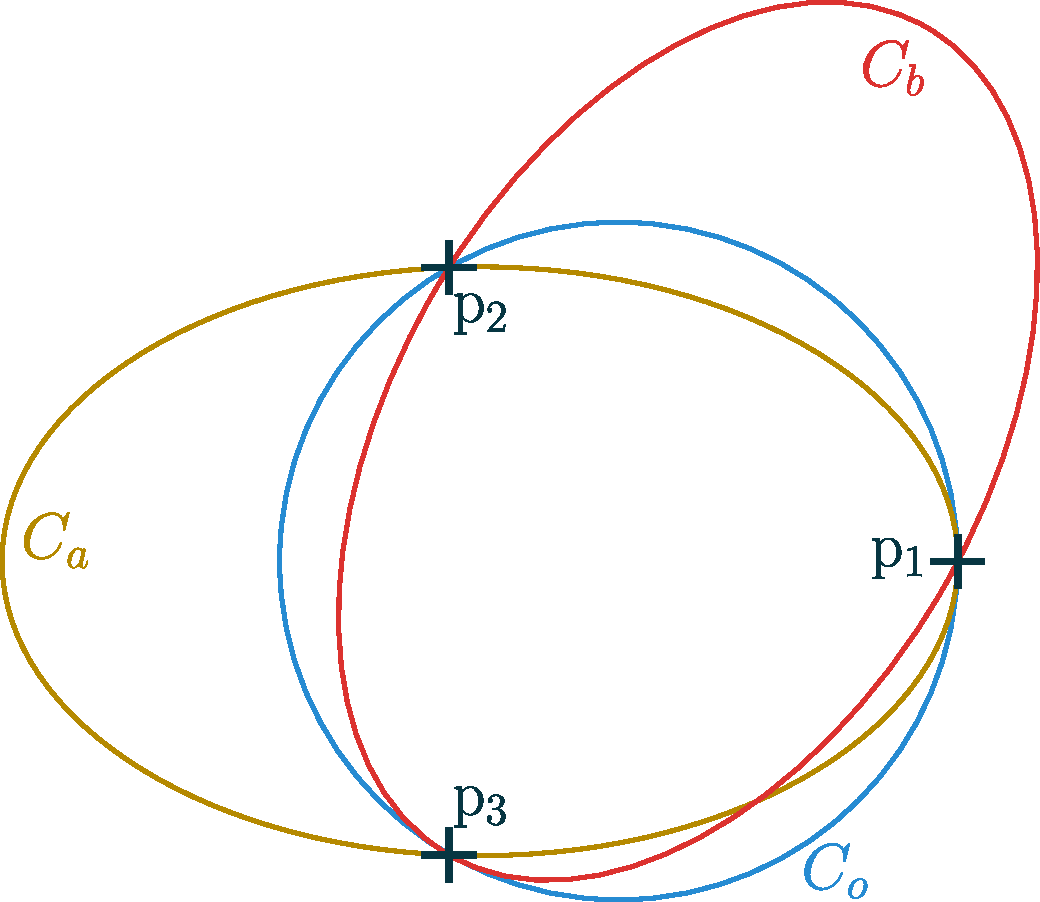
\includegraphics[width=0.63\linewidth]{3-conics-3-points}
    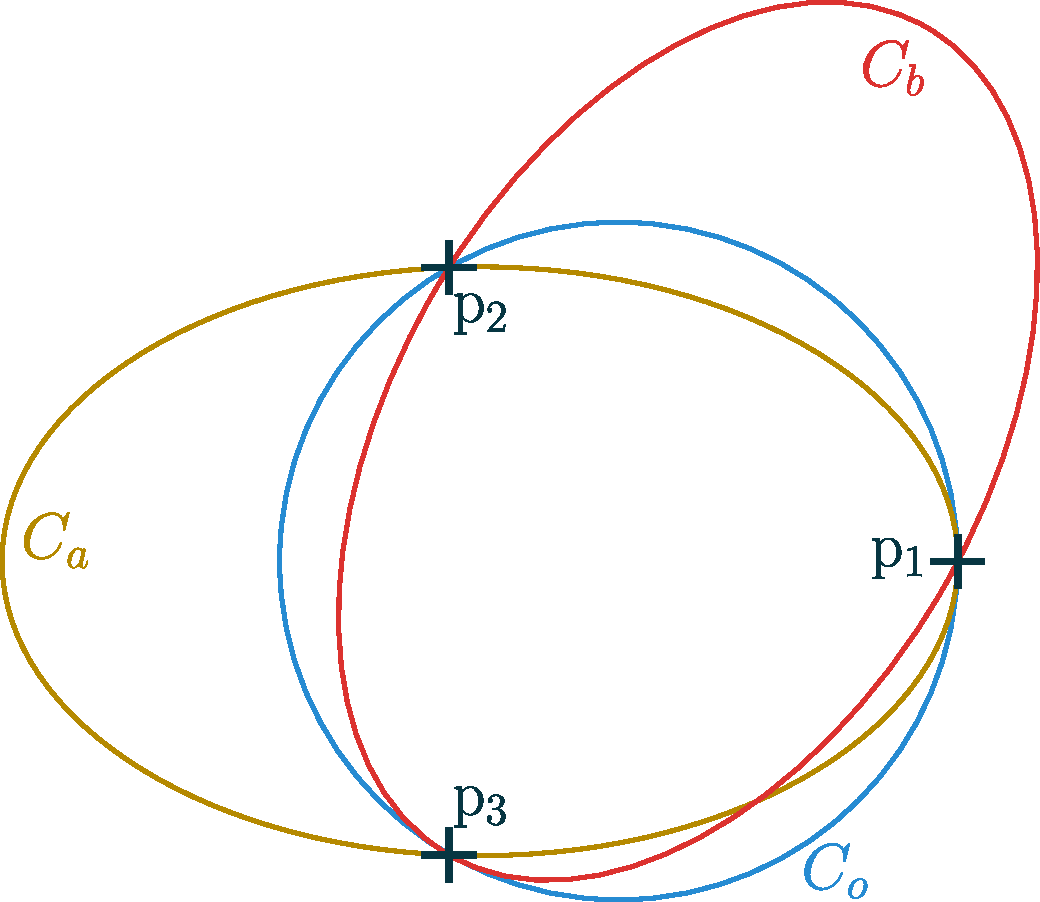
\includegraphics[width=0.5\linewidth]{3-conics-3-points}
    \caption{3 points \(\mathrm{p}_1\), \(\mathrm{p}_2\) and \(\mathrm{p}_3\) generating a 3-pencil \(\mathrm{Pencil}(C_o,C_a,C_b)\)}
\label{fig:3-pencil}
\end{figure}


Th.~\ref{th:n-points-generate-pencil}, illustrated by Fig.~\ref{fig:n-pencils}, presents a generalization of the case of four points generating a 2-pencils to $n$ points.


\begin{figure}[!ht]
    \centering
    \begin{subfigure}[t]{0.32\textwidth}
    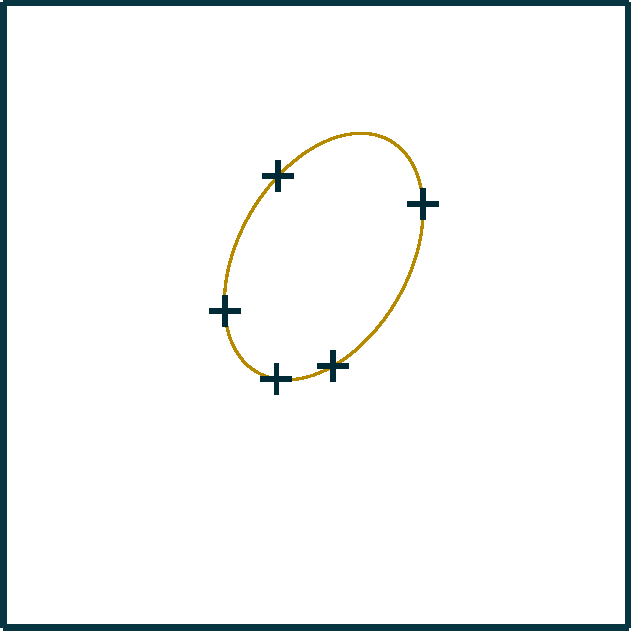
\includegraphics[width=\linewidth]{proj-3213256-pencil-1}
    \subcaption{\(1\)-pencil}\label{fig:n-pencils:1-pencil} 
    \end{subfigure}
    \begin{subfigure}[t]{0.32\textwidth}
    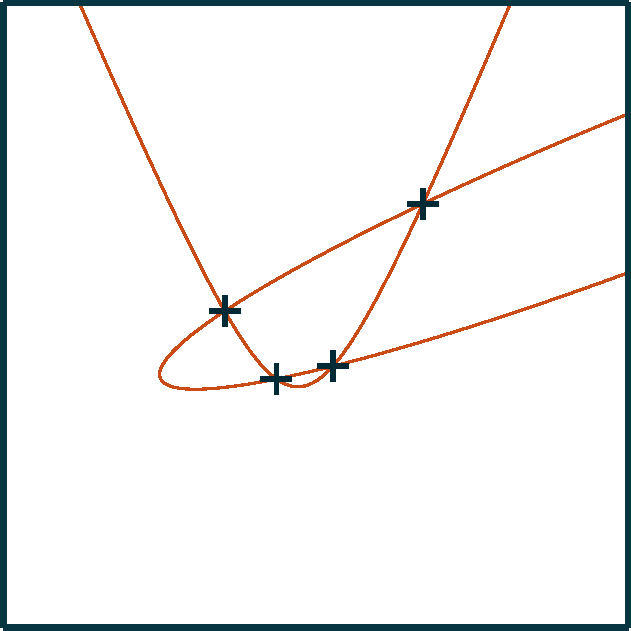
\includegraphics[width=\linewidth]{proj-3213256-pencil-2}
    \subcaption{\(2\)-pencil}\label{fig:n-pencils:2-pencil}
    \end{subfigure}
    \begin{subfigure}[t]{0.32\textwidth}
    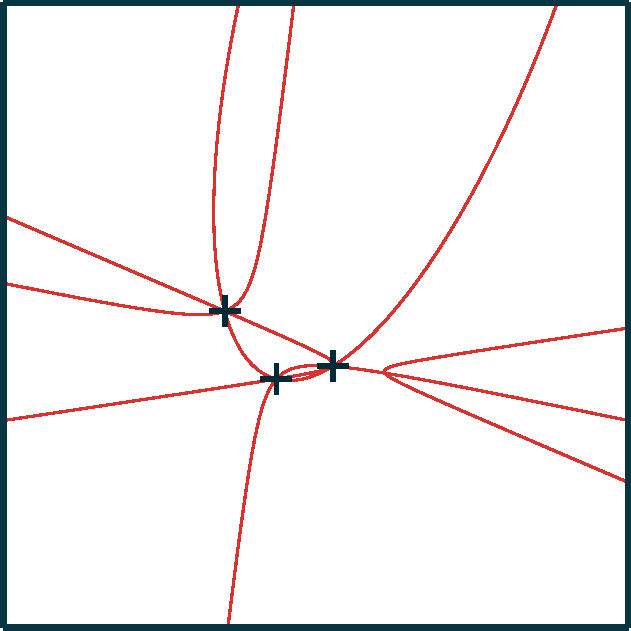
\includegraphics[width=\linewidth]{proj-3213256-pencil-3}
    \subcaption{\(3\)-pencil}\label{fig:n-pencils:3-pencil}
    \end{subfigure}
    \begin{subfigure}[t]{0.32\textwidth}
    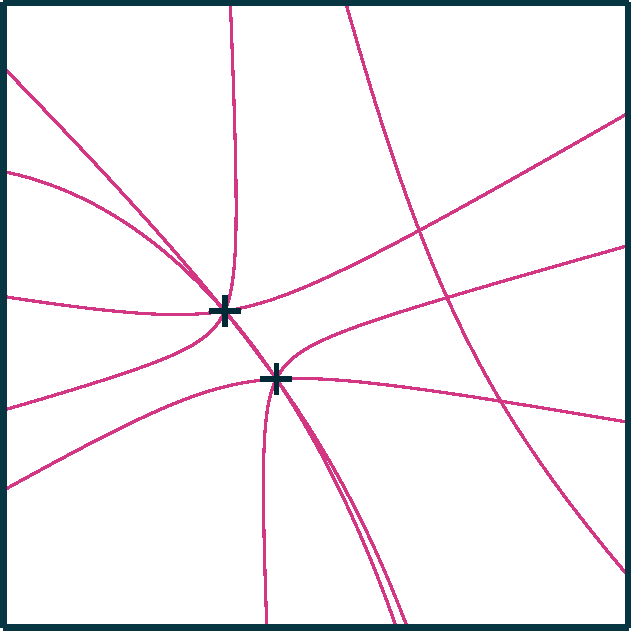
\includegraphics[width=\linewidth]{proj-3213256-pencil-4}    
    \subcaption{\(4\)-pencil}\label{fig:n-pencils:4-pencil}   
    \end{subfigure}
    \begin{subfigure}[t]{0.32\textwidth}
    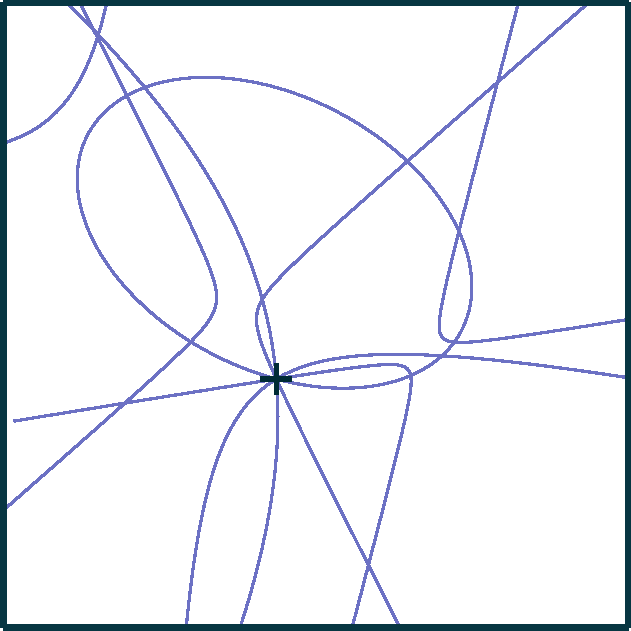
\includegraphics[width=\linewidth]{proj-3213256-pencil-5}
    \subcaption{\(5\)-pencil}\label{fig:n-pencils:5-pencil}   
    \end{subfigure}
    \begin{subfigure}[t]{0.32\textwidth}
    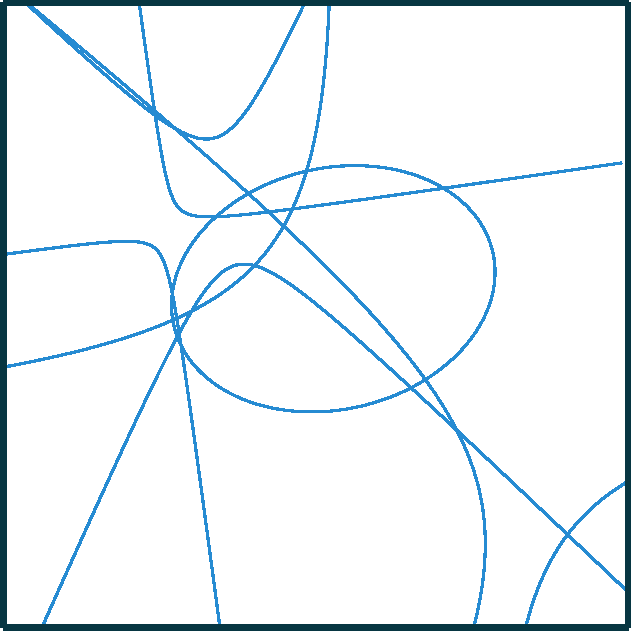
\includegraphics[width=\linewidth]{proj-3213256-pencil-6}
    \subcaption{\(6\)-pencil}\label{fig:n-pencils:6-pencil}   
    \end{subfigure}
    \captionsetup{subrefformat=parens}
     \caption{Some pencils of various orders represented by some random conics (among infinite), generated by 
     5~\subref{fig:n-pencils:1-pencil},
     4~\subref{fig:n-pencils:2-pencil}, 
     3~\subref{fig:n-pencils:3-pencil}, 
     2~\subref{fig:n-pencils:4-pencil}, 
     1~\subref{fig:n-pencils:5-pencil} and 
     0~\subref{fig:n-pencils:6-pencil} points.}\label{fig:n-pencils}
\end{figure}


\begin{theorem}\label{th:n-points-generate-pencil}
    A set of \(n\) linearly independent points generates a \((6-n)\)-pencil.
    Every conic passing through these $n$ points belongs to this pencil.
\end{theorem}

\begin{proof}
  As we work with a polynomial embedding described in Sec.~\ref{sec:conic-representation}, the points are vectors of dimension 6. Therefore, at most six points can be linearly independent.
    Consider \(6\) linearly independent points \((\mathrm{p}_1,\dots,\mathrm{p}_n\), \(\mathrm{q}_{1}, \dots,\mathrm{q}_{6-n})\) with \(n \leqslant 6\). 
    Five points are needed to build a conic. 
    There are \(6-n\) subset of \(5\) of the given points containing \(\mathrm{p}_1,\dots,\mathrm{p}_n\). We can then build exactly \(6-n\) linearly independent conics passing through \(\mathrm{p}_1,\dots,\mathrm{p}_n\), implying that \(n\) linearly independent points generate a \((6-n)\)-pencil.
\end{proof}




%%%%%%%%%%%%%%%%%%%%%%%%%%%%%%%%%%%%%%%%%%%%%%%%%%%%%%%%%%%%%%%%%%%%%%%%%%%%%%%%%%%%%%%%%%%%%%%%%%%%%%%%%%%%%
%%%%%%%%%%%%%%%%%%%%%%%%%%%%%%%%%%%%%%%%%%%%%%%%%%%%%%%%%%%%%%%%%%%%%%%%%%%%%%%%%%%%%%%%%%%%%%%%%%%%%%%%%%%%%

\subsection{Intersecting conics}
Two different conics \(C_a\) and \(C_b\) may have from zero to four real intersection points. Finding them is not a new problem, and two methods are usually encountered:
\begin{itemize}
    \item the use of Gröbner basis manipulation to get a quartic polynomial of one variable and finding its roots \cite{heck_birds-eye_2003},
    \item the extraction of a degenerate conic in \(Pencil(C_a, C_b)\), its factorization into two lines and intersecting them with \(C_a\) or \(C_b\)~\cite{richter-gebert_perspectives_2011}.
\end{itemize}

There are closed forms for the Gröbner basis method, but they imply fourth-degree polynomials subject to numerical instability, thus converging methods are preferred in practice. It is interesting to note that Faucette \cite{faucette_geometric_1996} gives a method to find the roots of any quartic polynomial of one variable by finding the intersection of two conics by using the degenerate conic method.% These two problems are equivalent. 

Richter-Gebert~\cite{richter-gebert_perspectives_2011} also investigated the degenerate conic method, but in a more complete way. The downside of Richter-Gebert's method is the use of complex objects, which could be avoided for the most part.


These section's results are adaptable to a Geometric Algebra context, a perspective that will be adopted and elaborated upon in the next section.


%%%%%%%%%%%%%%%%%%%%%%%%%%%%%%%%%%%%%%%%%%%%%%%%%%%%%%%%%%%%%%%%%%%%%%%%%%%%%%%%%%%%%%%%%%%%%%%%%%%%%%%%%%%%%
%%%%%%%%%%%%%%%%%%%%%%%%%%%%%%%%%%%%%%%%%%%%%%%%%%%%%%%%%%%%%%%%%%%%%%%%%%%%%%%%%%%%%%%%%%%%%%%%%%%%%%%%%%%%%
%%%%%%%%%%%%%%%%%%%%%%%%%%%%%%%%%%%%%%%%%%%%%%%%%%%%%%%%%%%%%%%%%%%%%%%%%%%%%%%%%%%%%%%%%%%%%%%%%%%%%%%%%%%%%
%%%%%%%%%%%%%%%%%%%%%%%%%%%%%%%%%%%%%%%%%%%%%%%%%%%%%%%%%%%%%%%%%%%%%%%%%%%%%%%%%%%%%%%%%%%%%%%%%%%%%%%%%%%%%
%%%%%%%%%%%%%%%%%%%%%%%%%%%%%%%%%%%%%%%%%%%%%%%%%%%%%%%%%%%%%%%%%%%%%%%%%%%%%%%%%%%%%%%%%%%%%%%%%%%%%%%%%%%%%
%%%%%%%%%%%%%%%%%%%%%%%%%%%%%%%%%%%%%%%%%%%%%%%%%%%%%%%%%%%%%%%%%%%%%%%%%%%%%%%%%%%%%%%%%%%%%%%%%%%%%%%%%%%%%
\section{QC2GA and GAC: two equivalent algebras}
\label{sec:QCGA_and_GAC}
%%%%%%%%%%%%%%%%%%%%%%%%%%%%%%%%%%%%%%%%%%%%%%%%%%%%%%%%%%%%%%%%%%%%%%%%%%%%%%%%%%%%%%%%%%%%%%%%%%%%%%%%%%%%%
\subsection{Conics and Geometric Algebra}

Upon reviewing Eq.~\eqref{eq:PMat} and Eq.~\eqref{eq:minors}, it becomes apparent that the matrix \(\mathrm{P}\) encapsulates not only the characteristics of the conic \(C\) but also those related to the evaluation point \(\mathrm{p}\).
Furthermore, Geometric Algebra allows computing the determinant of \(\mathrm{P}\) by wedging together vectors embedded by \(Q\) in \(\mathbb{G}_6\) of basis \((e_1, e_2, e_3, e_3, e_5, e_6)\), these vectors being analogous to the rows of the matrix \(\mathrm{P}\), as introduced in \(\bigwedge \mathbb{R}^6\)~\cite{a_kirillov_elements_1974,perwass_geometric_2009}. This also enables us to separate the point and conic terms into two different objects.
\begin{align}
Q(\mathrm{p}) &= x^2 e_1 + y^2 e_2 + xy e_3 + xw e_4 + yw e_5 + w^2 e_6 \\
C &= Q(\mathrm{p}_1) \wedge Q(\mathrm{p}_2) \wedge Q(\mathrm{p}_3) \wedge Q(\mathrm{p}_4) \wedge Q(\mathrm{p}_5) \\
\det(\mathrm{P}) I_6 &= C \wedge Q(\mathrm{p})
\end{align}
where \(I_6\) is the pseudoscalar of \(\mathbb{G}_6\).
The description of a conic in Eq.~\eqref{eq:PMat} is then equivalent to a simple exterior product between a conic \(C\) built from five points \(\mathrm{p}_1,\dots,\mathrm{p}_5\) and an evaluation point \(\mathrm{p}\). This results in a similar evaluation equation as in Eq.~\eqref{eq:conic_R6}.
\begin{equation}
C \wedge Q(\mathrm{p}) = 0
\end{equation}
Similarly to how the coefficients \((a,b,c,d,e,f)\) of the conic are stored in the conic object representation of Eq.~\eqref{eq:conic_R6}, we find that they are stored in the dual of the Geometric Algebra object \(C\) in Eq.~\eqref{eq:dual}. This property is the brick upon which algebras such as QCGA~\cite{breuils_three-dimensional_2019} or GAC~\cite{hrdina_geometric_2018} are built.
\begin{equation}\label{eq:dual}
    C^* = a e_1^c + b e_2^c + c e_3^c + d e_4^c + e e_5^c + f e_6^c
\end{equation}
This is the principle of Perwass' conic space \cite{perwass_geometric_2009}, which is then extended into the conformal conic space. In the conformal conic space - of basis \\\(\left(e_1,e_2,\bar n_1, n_1,\bar n_2, n_2,\bar n_3, n_3\right)\) - two more vectors are added in order to have three pairs of null vectors whose inner product results in \(-1\).
\begin{equation}
    \begin{tabular}{l|cccccccc}
    & \(e_1\)
    & \(e_2\)
    & \(\bar n_1\)
    & \(     n_1\)
    & \(\bar n_2\)
    & \(     n_2\)
    & \(\bar n_3\)
    & \(     n_3\) \\
    \hline
    \(e_1         \)  & 1 & . & . & . & . & . & . & . \\
    \(e_2         \)  & . & 1 & . & . & . & . & . & . \\
    \(\bar n_1    \)  & . & . & 0 &-1 & . & . & . & . \\
    \(     n_1    \)  & . & . &-1 & 0 & . & . & . & . \\
    \(\bar n_2    \)  & . & . & . & . & 0 &-1 & . & . \\
    \(     n_2    \)  & . & . & . & . &-1 & 0 & . & . \\
    \(\bar n_3    \)  & . & . & . & . & . & . & 0 &-1 \\
    \(     n_3    \)  & . & . & . & . & . & . &-1 & 0
    \end{tabular}
\end{equation}
Points and conics are then built as follows:
\begin{align}
    \mathrm{p} &=  \bar n_1 + \bar n_2 + x  e_1 + y e_2 + \cfrac{x^2}{2} n_1 + \cfrac{y^2}{2} n_2 + xy n_3\\
    C &= \mathrm{p}_1 \wedge \mathrm{p}_2 \wedge \mathrm{p}_3 \wedge \mathrm{p}_4 \wedge \mathrm{p}_5 \wedge \left(\bar n_1 - \bar n_2\right) \wedge \bar n_3 \\
    &= -2 a \bar n_1 - 2 b \bar n_2 - c \bar n_3+ d e_1 + e e_2 - \cfrac{f}{2} \left(n_1 + n_2\right)
\end{align}
%This algebra is the basis upon which are built the two algebras QC2GA and GAC.
This algebra forms the foundation of the two algebras QC2GA and GAC presented in the following section.


%%%%%%%%%%%%%%%%%%%%%%%%%%%%%%%%%%%%%%%%%%%%%%%%%%%%%%%%%%%%%%%%%%%%%%%%%%%%%%%%%%%%%%%%%%%%%%%%%%%%%%%%%%%%%
%%%%%%%%%%%%%%%%%%%%%%%%%%%%%%%%%%%%%%%%%%%%%%%%%%%%%%%%%%%%%%%%%%%%%%%%%%%%%%%%%%%%%%%%%%%%%%%%%%%%%%%%%%%%%
\subsection{Two-dimensional Quadric Conformal Algebra (QC2GA)}
\label{sec:qc2ga}
QC2GA is the 2D version of QCGA algebra by Breuils et al~\cite{breuils_three-dimensional_2019}.
QC2GA is built from the same signature as Perwass' algebra.
\begin{equation}
    \begin{tabular}{l|cccccccc}
    & \gavec{1}{}
    & \gavec{2}{}
    & \gavec{o}{1}
    & \gavec{\infty}{1}
    & \gavec{o}{2}
    & \gavec{\infty}{2}
    & \gavec{o}{3}
    & \gavec{\infty}{3} \\
    \hline
    \gavec{1}{}           & 1 & . & . & . & . & . & . & . \\
    \gavec{2}{}           & . & 1 & . & . & . & . & . & . \\
    \gavec{o}{1}          & . & . & 0 &-1 & . & . & . & . \\
    \gavec{\infty}{1}     & . & . &-1 & 0 & . & . & . & . \\
    \gavec{o}{2}          & . & . & . & . & 0 &-1 & . & . \\
    \gavec{\infty}{2}     & . & . & . & . &-1 & 0 & . & . \\
    \gavec{o}{3}          & . & . & . & . & . & . & 0 &-1 \\
    \gavec{\infty}{3}     & . & . & . & . & . & . &-1 & 0
    \end{tabular}
\end{equation}
QC2GA formalism relies on the following blades:
\begin{subequations}\label{eq:qc2ga-blades}
\begin{align}\displaystyle
&e_o = e_{o_1} + e_{o_2} &\forcenumbering&&
& e_{\infty} =  \frac{e_{\infty_1} + e_{\infty_2}}{2}\\
&I_o^\triangleright = \left(e_{o_1} - e_{o_2}\right) \wedge e_{o_3}   &\forcenumbering&\:&
&I_{\infty}^\triangleright\! =\! \left(e_{\infty_1}\! -\! e_{\infty_2}\right)\! \wedge\! e_{\infty_3} \\
&I_o = e_{o_1} \wedge e_{o_2} \wedge e_{o_3}   &\forcenumbering&&
&I_{\infty} = e_{\infty_1} \wedge e_{\infty_2} \wedge e_{\infty_3}  \\
&I_\epsilon = e_1 \wedge e_2   &\forcenumbering&&
&I = I_\epsilon \wedge I_{\infty} \wedge I_o
\end{align}
\end{subequations}
And QC2GA objects are constructed just like Perwass'.

\begin{align}\displaystyle
\qcgaobject{\mathrm{p}} &= e_o + x e_1 + y e_2 + x^2 \frac{ e_{\infty_1}}{2} + y^2 \frac{e_{\infty_2} }{2} + xy e_{\infty_3} \\
\qcgaobject{C} &= \qcgaobject{\mathrm{p}_1} \wedge \qcgaobject{\mathrm{p}_2} \wedge \qcgaobject{\mathrm{p}_3} \wedge \qcgaobject{\mathrm{p}_4} \wedge \qcgaobject{\mathrm{p}_5} \wedge I_o^\triangleright \\
\qcgaobject{C^*}  &= a (\frac{e_{\infty_1}}{2})^{-1} +  b (\frac{e_{\infty_2}}{2})^{-1} + c e_{\infty_3}^{-1} + d e_1^{-1} + e e_2^{-1} + f e_o^{-1} \\
&= - 2 a e_{o_1} - 2 b e_{o_2} - c e_{o_3} + d e_1 + e e_2 - f e_\infty
\end{align}
with \((a,b,c,d,e,f)\in\mathbb{R}^6\) the parameters of the conic \(C\) represented by \(\qcgaobject{C}\). QC2GA supports intersections of conics and provides the capability to evaluate if a point lies on a conic:
\begin{align} \displaystyle
\qcgaobject{Inter} = \qcgaobject{C_1} \vee \qcgaobject{C_2} = (\qcgaobject{C^*_1} \wedge \qcgaobject{C^*_2})^* \span \label{eq:antiwedge} \\ 
\qcgaobject{\mathrm{p}} \in \qcgaobject{C} &\iff \qcgaobject{\mathrm{p}}\wedge \qcgaobject{C} = 0 
\iff \qcgaobject{\mathrm{p}} \cdot (\qcgaobject{C^*}) = 0
\end{align}

%%%%%%%%%%%%%%%%%%%%%%%%%%%%%%%%%%%%%%%%%%%%%%%%%%%%%%%%%%%%%%%%%%%%%%%%%%%%%%%%%%%%%%%%%%%%%%%%%%%%%%%%%%%%%
%%%%%%%%%%%%%%%%%%%%%%%%%%%%%%%%%%%%%%%%%%%%%%%%%%%%%%%%%%%%%%%%%%%%%%%%%%%%%%%%%%%%%%%%%%%%%%%%%%%%%%%%%%%%%


\subsection{Geometric Algebra for Conics (GAC)}


GAC is an alternative Geometric Algebra for conics introduced by J.~Hrdina et al.~\cite{hrdina_geometric_2018}. Its basis, denoted as \(\left(e_1, e_2, \bar{n}_+, n_+, \bar{n}_-, n_-, \bar{n}_\times, n_\times\right)\), shares the same signature as QC2GA.
\begin{equation}
    \begin{tabular}{l|cccccccc}
    & \(e_1\)
    & \(e_2\)
    & \(\bar n_+\)
    & \(     n_+\)
    & \(\bar n_-\)
    & \(     n_-\)
    & \(\bar n_\times\)
    & \(     n_\times\) \\
    \hline
    \(e_1           \)  & 1 & . & . & . & . & . & . & . \\
    \(e_2           \)  & . & 1 & . & . & . & . & . & . \\
    \(\bar n_+      \)  & . & . & 0 &-1 & . & . & . & . \\
    \(     n_+      \)  & . & . &-1 & 0 & . & . & . & . \\
    \(\bar n_-      \)  & . & . & . & . & 0 &-1 & . & . \\
    \(     n_-      \)  & . & . & . & . &-1 & 0 & . & . \\
    \(\bar n_\times \)  & . & . & . & . & . & . & 0 &-1 \\
    \(     n_\times \)  & . & . & . & . & . & . &-1 & 0
    \end{tabular}
\end{equation}
In GAC, points and conics are defined as follows:
\begin{align}\displaystyle
\gacobject{\mathrm{p}} &= \bar n_{+} + x e_1 + y e_2 + \frac{x^2 + y^2}{2} n_{+} + \frac{x^2 - y^2}{2} n_{-} + xy  n_{\times}  \\
\gacobject{C} &= \gacobject{\mathrm{p}_1} \wedge \gacobject{\mathrm{p}_2} \wedge \gacobject{\mathrm{p}_3} \wedge \gacobject{\mathrm{p}_4} \wedge \gacobject{\mathrm{p}_5}\wedge \bar n_- \wedge \bar n_\times\\
\gacobject{C^*}&= -  (a+b) \bar n_{+} -  (a-b) \bar n_{-} - c \bar n_{\times} + d e_1 + e e_2 - f n_{+} 
\end{align}
The way GAC is used in practice is identical to QC2GA.
\begin{align}\displaystyle % \span is used to fuse two cells somehow
\gacobject{Inter} = \gacobject{C_1} \vee \gacobject{C_2} = (\gacobject{C^*_1} \wedge \gacobject{C^*_2})^* \span \\ 
\gacobject{\mathrm{p}} \in \gacobject{C} &\iff \gacobject{\mathrm{p}}\wedge \gacobject{C} = 0 \iff \gacobject{\mathrm{p}} \cdot (\gacobject{C^*}) = 0
\end{align}
\(\gacobject{Inter}\) represents the intersection of conics \(\gacobject{C_1}\) and \(\gacobject{C_2}\). Here \(\gacobject{\mathrm{p}} \in \gacobject{C}\) means that the point \(\gacobject{\mathrm{p}}\) lies on the conic \(\gacobject{C}\).

%%%%%%%%%%%%%%%%%%%%%%%%%%%%%%%%%%%%%%%%%%%%%%%%%%%%%%%%%%%%%%%%%%%%%%%%%%%%%%%%%%%%%%%%%%%%%%%%%%%%%%%%%%%%%
%%%%%%%%%%%%%%%%%%%%%%%%%%%%%%%%%%%%%%%%%%%%%%%%%%%%%%%%%%%%%%%%%%%%%%%%%%%%%%%%%%%%%%%%%%%%%%%%%%%%%%%%%%%%%
%%%%%%%%%%%%%%%%%%%%%%%%%%%%%%%%%%%%%%%%%%%%%%%%%%%%%%%%%%%%%%%%%%%%%%%%%%%%%%%%%%%%%%%%%%%%%%%%%%%%%%%%%%%%%
%%%%%%%%%%%%%%%%%%%%%%%%%%%%%%%%%%%%%%%%%%%%%%%%%%%%%%%%%%%%%%%%%%%%%%%%%%%%%%%%%%%%%%%%%%%%%%%%%%%%%%%%%%%%%
%%%%%%%%%%%%%%%%%%%%%%%%%%%%%%%%%%%%%%%%%%%%%%%%%%%%%%%%%%%%%%%%%%%%%%%%%%%%%%%%%%%%%%%%%%%%%%%%%%%%%%%%%%%%%
%%%%%%%%%%%%%%%%%%%%%%%%%%%%%%%%%%%%%%%%%%%%%%%%%%%%%%%%%%%%%%%%%%%%%%%%%%%%%%%%%%%%%%%%%%%%%%%%%%%%%%%%%%%%%

\subsection{GAC and QC2GA are equivalent}
\label{sec:equivalence}
GAC and QC2GA have been proved equivalent~\cite{chomicki_intersection_2023}. This section goes further with a focus on the translators of both algebras.

GAC and QC2GA share the same metric, and at a first glance, their objects appear to be similar. A closer view of their construction can demonstrate that they are isomorphic. Notably, one can express the basis vectors of GAC using those of QC2GA, demonstrating an isomorphism between QC2GA and GAC objects. 
\begin{align}\displaystyle\label{eq:equivalence_start}
\bar n_{+} &= e_{o_1} + e_{o_2} && \forcenumbering &
\bar n_{-} &= e_{o_1} - e_{o_2} && \forcenumbering &
\bar n_{\times} &= e_{o_3}\\
n_{+} &= \frac{e_{\infty_1} + e_{\infty_2}}{2} && \forcenumbering &
n_{-} &= \frac{e_{\infty_1} - e_{\infty_2}}{2} && \forcenumbering &
n_{\times} &= e_{\infty_3}\\
            \gacobject{\mathrm{p}} &= e_o + xe_1 + ye_2 + \frac{x^2 e_{\infty_1} + y^2 e_{\infty_2}}{2}+xye_{\infty_3}
            = \qcgaobject{\mathrm{p}} \span\span\span\span\span\span\span\span\\
            \gacobject{C} &= - 2a e_{o_1} -  2b e_{o_2}- c e_{o_3} + d e_1 + e e_2 - f e_\infty
            = \qcgaobject{C} \span\span\span\span\span\span\span\span
            \label{eq:equivalence_end}
\end{align}
%Since they are equivalent, they share their respective properties.
Eqs.~(\ref{eq:equivalence_start}-\ref{eq:equivalence_end}) show by construction that QC2GA and GAC only differ by a change of basis.
Such a result can bring together all the research and developments related to both algebras so that they share their respective properties. GAC possesses versors that facilitate operations such as rotation, translation, dilation, and even a form of "general reflection" (resembling CGA's spherical inversion~\cite{perwass_geometric_2009}, but using conics). On the other hand, QC2GA also encompasses rotations and translations (directly inherited from Perwass' conformal conic algebra) and expresses its translator in a more straightforward way than GAC. Since these two algebras are equivalent, tools and techniques from both GAC and QC2GA can be seamlessly interchanged. 

~\\
For instance, GAC translators of displacement \((u,v)\) are of the form:
%    # GAC
    % \begin{align}
    % T_{x_+} &= 1 - \frac{u}{2} e_1\wedge n_+  &
    % T_{y_+} &= 1 - \frac{v}{2} e_2\wedge n_+ \\
    % T_{x_-} &= 1 - \frac{u}{2} e_1\wedge n_-  - \frac{u^2}{4} n_+\wedge n_-  &
    % T_{y_-} &= 1 + \frac{v}{2} e_2\wedge n_- - \frac{v^2}{4} n_+\wedge n_-  \\
    % T_{x_\times} &= 1 - \frac{u}{2} e_2\wedge n_\times &
    % T_{y_\times} &= 1 - \frac{v}{2} e_1\wedge n_\times \\
    % T_{GAC_x} &= t_{x_+} t_{x_-} t_{x_\times} &
    % T_{GAC_y} &= t_{y_+} t_{y_-} t_{y_\times} \\
    % T_{GAC} &= t_{GAC_x} t_{GAC_y}
    % \end{align}



    \begin{align}
    &T_{x_+} = 1 - \frac{u}{2} e_1\wedge n_+  &
    &T_{y_+} = 1 - \frac{v}{2} e_2\wedge n_+ \\
    &T_{x_-} = 1 - \frac{u}{2} e_1\wedge n_-  - \frac{u^2}{4} n_+\wedge n_-  & ~~~
    &T_{y_-} = 1 + \frac{v}{2} e_2\wedge n_- - \frac{v^2}{4} n_+\wedge n_-  \\
    &T_{x_\times} = 1 - \frac{u}{2} e_2\wedge n_\times &
    &T_{y_\times} = 1 - \frac{v}{2} e_1\wedge n_\times \\
    &T_{GAC_x} = t_{x_+} t_{x_-} t_{x_\times} &
    &T_{GAC_y} = t_{y_+} t_{y_-} t_{y_\times} \\
    &T_{GAC} = t_{GAC_x} t_{GAC_y}
    \end{align}
But Perwass' translators are of the form:
%    # PERWASS
    \begin{align}
    T_{x_1} &= 1 - \frac{u}{2} e_{1\infty_1} &
    T_{y_1} &= 1 - \frac{v}{2} e_{2\infty_2} \\
    T_{x_2} &= 1 - \frac{u}{2} e_{2\infty_3} &
    T_{y_2} &= 1 - \frac{v}{2} e_{1\infty_3} \\
    T_{QC2GA_x} &= t_{x_2} t_{x_1} &
    T_{QC2GA_y} &= t_{y_2} t_{y_1} \\
    T_{QC2GA} &= t_{QC2GA_x} t_{QC2GA_y}
    \end{align}
Both have the \(x\) and the \(y\) translators separated, but in the end, QC2GA's translator is simpler and more computationally efficient. Hence, now anyone working in GAC could use this translator instead, and symmetrically, anyone working in QC2GA can now use any versor that was not implemented in QC2GA, such as general conic reflection.

Therefore, in the following sections of this paper, the labels "QC2GA" and "GAC" on top of geometric objects will be omitted, as this paper will adhere to the formalism of QC2GA. It is important to keep in mind that every property relevant to QC2GA also directly applies to GAC.


%%%%%%%%%%%%%%%%%%%%%%%%%%%%%%%%%%%%%%%%%%%%%%%%%%%%%%%%%%%%%%%%%%%%%%%%%%%%%%%%%%%%%%%%%%%%%%%%%%%%%%%%%%%%%%%%%%%%%%%%%%%%%%%%%%%%%%%%%%%%%%%%%%%%%%%%%%%%%%%%%%%%%%%%%%%%%%%%%%%%%%%%%%%%%%%%%%%%%%%%%%%%%%%%%%
%%%%%%%%%%%%%%%%%%%%%%%%%%%%%%%%%%%%%%%%%%%%%%%%%%%%%%%%%%%%%%%%%%%%%%%%%%%%%%%%%%%%%%%%%%%%%%%%%%%%%%%%%%%%%
%%%%%%%%%%%%%%%%%%%%%%%%%%%%%%%%%%%%%%%%%%%%%%%%%%%%%%%%%%%%%%%%%%%%%%%%%%%%%%%%%%%%%%%%%%%%%%%%%%%%%%%%%%%%%
%%%%%%%%%%%%%%%%%%%%%%%%%%%%%%%%%%%%%%%%%%%%%%%%%%%%%%%%%%%%%%%%%%%%%%%%%%%%%%%%%%%%%%%%%%%%%%%%%%%%%%%%%%%%%
%%%%%%%%%%%%%%%%%%%%%%%%%%%%%%%%%%%%%%%%%%%%%%%%%%%%%%%%%%%%%%%%%%%%%%%%%%%%%%%%%%%%%%%%%%%%%%%%%%%%%%%%%%%%%
\section{Extending points in QC2GA}
\label{sec:points}

Sec.~\ref{sec:qc2ga} defines the concepts of points and conics in QC2GA. 
However, there are further distinctions to be made. Within this framework, the space of points implies several kinds of objects: points, imaginary points, and point-space elements. These objects are used to construct and manipulate various kinds of objects.

\begin{definition}[Point-Space Element]
A Point-Space Element of grade \(k\), or \(k\)-PSE, is a \(k\)-vector built from the basis
\begin{equation}
    \mathcal{B}_\mathrm{p} = \left(e_o, e_1, e_2, e_{\infty_1}, e_{\infty_2}, e_{\infty_3}\right)
\end{equation}
Let \(\mathrm{PSE} = \bigwedge \mathcal{B}_\mathrm{p}\) denote the set of PSE and \(\mathrm{PSE}_k = \bigwedge_k \mathcal{B}_\mathrm{p}\) the set of \(k\)-PSE.
\label{def:Bp}
\end{definition}
\begin{definition}[Points]
A point is a \(1\)-PSE representing a location on the plane. The set of all points is the following:
\begin{equation}
\mathrm{Points} = \left\{e_o + x e_1 + y e_2 + \frac{1}{2}\left(x^2 e_{\infty_1} + y^2  e_{\infty_2}\right) + xy e_{\infty_3}, (x,y)\in\mathbb{R}^2\right\}
\end{equation}
\end{definition}
\begin{definition}[Point at infinity]\label{def:pt_inf}
A point at infinity is a \(1\)-PSE representing a location on the line at infinity. The set of all points at infinity is the following:
\begin{equation}
    \mathrm{Points}_{\infty} = \left\{x^2 e_{\infty_1} + y^2 e_{\infty_2} + 2 xy e_{\infty_3}, (x,y)\in\mathbb{R}^2\right\}
\end{equation}
\end{definition}
Points at infinity are often met when working in projective geometry and conics~\cite{richter-gebert_perspectives_2011}. Points at infinity are common in the context of quadratic primitives and geometric algebra ~\cite{hrdina_geometric_2018,breuils_three-dimensional_2019} and are described in a recent paper as the meeting point of two parallel line~\cite{2024-01-09louckaAlgorithmsConicFitting}. Def.~\ref{def:pt_inf} presents points at infinity as characterised by an angle, which is the same thing.
\begin{definition}[Imaginary Point-Space Element]
A \(k\)-PSE \(A\) is said to be imaginary if and only if there is no point \(\mathrm{p}\) and \((k-1)\)-PSE \(B\) so that \({A=B\wedge\mathrm{p}}\).
%An imaginary PSE is a PSE from which no point can be factored with the outer product. 
In other words, an Imaginary Point-Space Element of grade \(k\) is not factorizable by the wedge product of a point and a \((k-1)\)-PSE.
The set of imaginary PSE of grade \(k\) is denoted by \(\mathrm{ImPSE}_k\).
\end{definition}
\begin{definition}[Real Point-Space Element]
A real \(k\)-PSE, is a PSE that can be expressed as the outer product of \(k\) points.
The set of real PSE of grade \(k\) is denoted \(\mathrm{RePSE}_k\).
For convenience, \(k\)-PSE will sometimes be denoted \(\mathrm{p}^k\).
\end{definition}
\begin{example}
Consider points \(\mathrm{p}\), \(\mathrm{p}_1\), \(\mathrm{p}_2\), \(\mathrm{p}_3\).
\begin{align}
e_{12} && \mbox{imaginary PSE} \\
\mathrm{p} \wedge e_{12} && \mbox{neither an imaginary nor a real PSE} \\
\mathrm{p}_1\wedge\mathrm{p}_2\wedge\mathrm{p}_3 && \mbox{real PSE}    
\end{align}
\end{example}

Points and real PSEs correspond to finite space locations and thus can be represented geometrically. Conversely, imaginary PSEs, which do not fall within this range, typically lack a concrete geometric interpretation, yet they remain useful in constructing and constraining pencils. Points at infinity, situated on the line at infinity, are defined solely by their direction. They represent the extrapolation of points projected towards infinity and are a unique category of imaginary \(1\)-PSE with actual geometric significance.

\begin{theorem}\label{th:sum-of-2-point-is-imaginary}
    The sum of two points can only be an imaginary \(1\)-PSE.
\end{theorem}

\begin{proof}
    For this proof, we operate in \(\mathbb{R}^6\).
    The linear space formed by two \(1\)-PSE is a line of \(\mathbb{R}^6\).
    The set \(\mbox{Points}\) is a quadratic surface.
    Finding the intersection between that line and the set of points is then done by finding the root of a quadratic polynomial of one variable, because a line is a one-dimensional object.
    This means that one can find at most two intersection points between \(\mbox{Points}\) and the line. This property is illustrated in Fig.\ref{fig:real_pt_space_slice}.
\end{proof}
\begin{figure}[ht!] 
    \begin{center}
    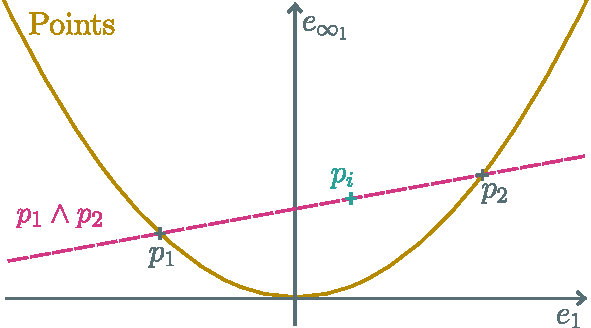
\includegraphics[width=0.6\linewidth]{real_point_space_e1i1}
    \end{center}
    \caption{A cut of the set \(\textrm{Points}\) along the plane \(e_{1}\wedge e_{\infty_1}\) with two points \(\mathrm{p}_1\) and \(\mathrm{p}_2\).
    The points generate the vector space \(\mathrm{p}_1\wedge \mathrm{p}_2\) containing one imaginary \(1\)-PSE~\(\mathrm{p}_i\).}
 \label{fig:real_pt_space_slice}
\end{figure}
% Understanding a six dimensional space is not really possible, but this theorem gives some hints to grasp the shape of \(\mathrm{Points}\) in the space of \(1\)-PSE. 
Th.~\ref{th:sum-of-2-point-is-imaginary} gives a grasp of the shape of the quadric surface Points within the space of \(1\)-PSE. The opposite is, of course, not true: \(e_1\) and \(e_2\) are two imaginary \(1\)-PSE, but they are not enough to construct a point. This means that there exist lines passing through two imaginary \(1\)-PSE passing through some holes on the surface of Points. 

All these definitions and theorems present a more generalized conception of points in QC2GA. These notions are used in the following section to properly define and manipulate pencils in QC2GA.
%%%%%%%%%%%%%%%%%%%%%%%%%%%%%%%%%%%%%%%%%%%%%%%%%%%%%%%%%%%%%%%%%%%%%%%%%%%%%%%%%%%%%%%%%%

\section{Conics and their pencils}
\label{sec:pencils}

This section redefines the concept of conics and pencils in QC2GA using the concept of Point-Space element introduced in Sec.~\ref{sec:points}.
\subsection{Right complement, orthogonality, and norm}

%A few general tools are to be defined in order to continue.
The right-complement operator, as introduced by~\cite{gunn2022bit}, has various definitions. In this paper, the following definition is used.
\begin{definition}[Right Complement]
The right complement operator of an algebra \(\mathbb{G}\) of dimension \(d\) is a linear map associating any k-vector \(E\) of the canonical algebraic basis \(\overline{\mathbb{G}}\) to the unique \((d-k)\)-vector \(E^c\) so that \(E\wedge E^c = I\). 
% Assume \(\matbb{G}\) a \(d\)-dimensional Geometric Algebra of canonical basis \(\overline{\mathbb{G}}\). The right complement of any canonical \(k\)-vector \(E=e_{i_1,\dots,i_k}\) is the \(d-k\)-vector \(E^c = \pm e_{j_1,\dots,j_{d-k}}\) so that \(E\wedge E^c = I\).
\end{definition}

\begin{example}
    Consider the algebra \(\mathbb{G}_3\) with canonical basis \(\big(e_1,e_2,e_3\big)\) and canonical algebraic basis \(\big(1,e_1,e_2,e_3,e_{12},e_{23},e_{31},e_{123}\big)\).  Then the right complement gives the following mapping:
%    Consider the algebra \(\mathbb{G}_3\) of basis \((e_1,e_2,e_3)\).
    \begin{align}
            1^c &=  e_{123} & e_{123}^c &= 1     \\
        e_{1}^c &=  e_{23}  &  e_{23}^c &=  e_{1} \\
        e_{2}^c &= -e_{13}  &  e_{13}^c &= -e_{2} \\
        e_{3}^c &=  e_{12}  &  e_{12}^c &=  e_{3} 
    \end{align}
     Since every multivector is a linear sum of elements of the canonical algebraic basis, 
%        Every multivector is a linear sum of elements of the canonical basis, hence the right complement can be used on any multivector.
    \begin{align}
                2^c &= 2 \times 1^c =   2 e_{123} \\
        (4 e_{1})^c &=  4 e_{23}   \\
        (5e_{2} + 7e_{12})^c &= -5e_{13} + 7e_{3} 
    \end{align}
\end{example}

\begin{remark}
Consider a multivector \(A=\sum_{E\in\overline{\mathbb{G}}} A_E E\) in \(\mathbb{G}\). The right complement of \(A\) is by linearity
\begin{align}
    A^c &= \sum_{E\in\overline{\mathbb{G}}} A_E E^c
\end{align}
\end{remark}


In other algebras, the norm of a multivector A is often defined as \(\sqrt{\tilde A \cdot A}\) where $\tilde A$ is the reverse of $A$~\cite{dorst_geometric_2010}. In QC2GA, this definition is not sufficient for many objects. For instance, the norm \(\sqrt{\tilde C \cdot C}\) applied to a conic \(C\) of parameters \((a,b,c,d,e,f)\) results in \( -2 a f - 2 b f + d^2 + e^2\), which is missing the term~\(c\). The term \(c\) is missing because of the term in \(e_{o_3}\) in the dual conic, which is lacking a \(e_{\infty_3}\) counterpart. Also, this expression lacks meaning and can sometimes be zero for conics such as some hyperbolas centered on the origin. These problems were a motivation to propose another definition of the norm.


\begin{definition}[Norm of a multivector of QC2GA]
    The norm \(\|A\|\) of a multivector of QC2GA \(A=\sum_{E\in\overline{\mathbb{G}}} A_E E\) is  
    \begin{equation}
        \|A\| = \sqrt{\left(A \wedge A^c\right)^*}= \sqrt{A^* \cdot A^c} = \sqrt{\sum_{E\in\overline{\mathbb{G}}} A_E^2}
    \end{equation}
Note that this norm embeds both the right complement and the dual.
\end{definition}


\begin{definition}[Orthogonality of multivectors] \label{def:orthogonalconics}
    Two multivectors \(A\) and \(B\) are orthogonal iff \(A \wedge B^c = 0\).
\end{definition}
\noindent Note that this definition of orthogonality is similar to~\cite{gunn2022bit} (section 5.1.2).

    
\subsection{Conics and their right complements}
\begin{definition}[Conic]
A conic is a blade of grade 7 of the form
\begin{align}
    C &= I^\triangleright_o \wedge \mathrm{p}_1 \wedge \mathrm{p}_2 \wedge \mathrm{p}_3 \wedge \mathrm{p}_4 \wedge \mathrm{p}_5 & \mbox{with }\mathrm{p}_1, \mathrm{p}_2, \mathrm{p}_3,\mathrm{p}_4,\mathrm{p}_5 \in \mathrm{PSE}_{1}
\end{align}
\end{definition}
\begin{definition}[Dual conic]
    A dual conic is the dual of a conic.
    It is a \(1\)-vector constructed on the basis \(\mathcal{B}_C=(e_{o_1},e_{o_2},e_{o_3},e_{1},e_{2},e_{\infty})\)
\end{definition}
\begin{theorem}\label{th:complement-1-PSE} 
The right complement of any non-zero \(1\)-PSE \(\mathrm{p}\) is a conic \(C\) so that ${C\wedge \mathrm{p} \ne 0}$.
\end{theorem}
\begin{proof}
This proof consists of doing the right complement of a \(1\)-PSE, observing through its dual that the result is a conic, and then wedging the conic with the \(1\)-PSE to get something proportional to the norm of the \(1\)-PSE.
\begin{align*}
\mathrm{p} &=a e_o + b e_1 + c e_2 + d e_{\infty_1} + e e_{\infty_2} + f e_{\infty_3} \neq 0\\
%\left(\mathrm{p}^c\right)^* &=a e_\infty + b e_1 + c e_2 + d e_{o_1} + e e_{o_2} + f e_{o_3} & \mbox{(dual conic)}\\
C=\mathrm{p}^c &= \left(a e_\infty + b e_1 + c e_2 + d e_{o_1} + e e_{o_2} + f e_{o_3}\right)^* & C \mbox{ is a conic}\\
\mathrm{p} \wedge \mathrm{p}^c &= \left(a^2 + b^2 +c^2 + d^2 + e^2 + f^2\right) I \ne 0
\end{align*}
\end{proof}


\begin{theorem}
The right complement of any conic \(C\) different than 0 is a \(1\)-PSE~\(\mathrm{p}\) so that ${C\wedge \mathrm{p} \ne 0}$.
\end{theorem}
\begin{proof}
\(\mathrm{p}^c = C\) therefore Th.~\ref{th:complement-1-PSE} applies.
\end{proof}
The right complement establishes a bijective duality between \(1\)-PSE and conics.
 %




\subsection{Pencils and their constraints}
This section introduces pencils as QC2GA objects, presents an elegant way to create and manipulate them, and also generalizes every object of QC2GA as either a pencil or a PSE.

\begin{definition}[Pencil]
    A \(n\)-pencil is the anti-outer product of \(n\) conics, which is the dual of a \(n\)-blade built on the basis 
    \begin{equation}
        \mathcal{B}_c = \left(e_{o_1},e_{o_2},e_{o_3},e_1,e_2,e_\infty\right)   
    \end{equation}
    In practice, a \(n\)-pencil is the intersection of the \(n\) conics. More precisely, a $n$-pencil is the vector space generated by $n$ conics.
\end{definition}
\begin{remark}
    A conic is a \(1\)-pencil.
\end{remark}
\noindent For pencils, we rely on two different kinds of null space representation, similarly to what can be found in Perwass' work~\cite{perwass_geometric_2009}.
%The Outer Product Null Space representation (OPNS), where \(a\) is said in \(A\) iif \(a \wedge A = 0\), and the Anti-outer Product Null Space representation (APNS), where \(a\) is said in \(A\) iif \(a \vee A = 0\).
\begin{definition}[Outer-Product Null Space]
The outer-product null space (OPNS) of a \(n\)-pencil \(P\), denoted \(\mathbb{NO}\left(P\right)\) is defined as 
\begin{equation}
    \mathbb{NO}\left(P\right) = \left\{A \in \bigcup_{i\in[0,6-n]}\mathrm{PSE}_{i} ~\middle|~ P \wedge A = 0 \right\}
\end{equation}
\end{definition}

\begin{definition}[Anti-outer-Product Null Space]
The anti-outer-product null space (APNS) of a \(n\)-pencil \(P\), denoted \(\mathbb{NA}(P)\) is defined as 
\begin{equation}
    \mathbb{NA}\left(P\right) = \left\{P' \in \bigcup_{i\in[0,n]}\mathrm{Pencils}_{i} ~\middle|~ P \vee P' = 0 \right\}
\end{equation}
with \(\vee\) the anti-outer product defined in Eq.~\ref{eq:antiwedge}.
\end{definition}

\noindent The APNS representation of a pencil is used to consider the pencil as a set of conics, and the OPNS representation of a pencil is used to consider a pencil as a set of PSE.
For simplicity, we consider that a PSE belongs to a pencil if and only if it belongs to its OPNS, and a pencil is included in another pencil if and only if it belongs to its APNS representation.

The blade \(I_o^\triangleright\) from Eqs.~\eqref{eq:qc2ga-blades} plays a central role in QCGA. It could be considered as "just" the two missing vectors to complete the point basis \(\mathcal{B}_\mathrm{p}\) from Def.~\eqref{def:Bp} into the full QC2GA, but it is possible to instead find a geometrical meaning for that blade.

\begin{theorem}
\(I_o^\triangleright\) is the pencil of all conics, namely, the vector space generated by all the conics.
\end{theorem}
\begin{proof}
\((I_o^\triangleright)^* = e_1\wedge e_2 \wedge e_{o_1} \wedge e_{o_2} \wedge e_{o_3} \wedge e_{\infty}\) therefore, any element of \(\mathcal{B}_C\) is in \((I_o^\triangleright)^*\), hence any dual conic is in \((I_o^\triangleright)^*\).
\end{proof}
That fundamental pencil \(I^\triangleright_o\) can then be constrained and extended with conics, PSE and their right complement.


%\textcolor{violet}{
\begin{theorem}\label{th:complement-n-PSE} 
The right complement of any \(n\)-PSE \(A \neq 0 \) is a \((6-n)\)-pencil \(P\) so that \(P \wedge A \ne 0\).
% \textcolor{violet}{The right complement of any \(n\)-PSE \(\mathrm{p}\) different than 0 is a \((6-n)\)-pencil \(P\) so that \(p \notin P\)}.
\end{theorem}
\begin{proof}
Let \(A\) be a \(n\)-PSE of coordinates \(\left(A_E\right)_{E\in \overline{\mathrm{PSE}_n}}\).
\begin{align*}
A &= \sum_{E\in \overline{\mathrm{PSE}_n}} A_E E \\
P &= A^c & \parbox{0.5\linewidth}{\(P\) is a pencil since dual of blade of \(\mathcal{B}_C\), ie dual of outer prod. of dual conics, ie anti-outer prod. of conics} \\
A\wedge P  &= \underbrace{\left(\sum_{E\in \overline{\mathrm{PSE}_n}} A_E^2\right)}_{> 0} I \ne 0
\end{align*}
\end{proof}
%}


%\textcolor{violet}{
\begin{theorem}
The right complement of any \(n\)-pencil \(P\) is a \((6-n)\)-PSE \(A\) so that \(A \notin P\).
\end{theorem}
%}
\begin{proof}
\(\mathrm{p}^c = P\) therefore Th.~\ref{th:complement-n-PSE} applies.
\end{proof}


\begin{theorem} \label{th:constraint-add-conic}
Let \(P\) be a pencil of order \(k\) and \(C\) be a conic not in \(P\).
    \(P\vee C\) is the pencil of order $k+1$ generated by all the conics of \(P\) and \(C\), where the operator~$\vee$ is defined in Eq.~\eqref{eq:antiwedge}.
\end{theorem}


\begin{proof}
Let \(P\) be a \(n\)-pencil and \(C\) a conic not in \(P\). 
\(P\) is the result of the meet product of \(n\) conics \(C_1, \dots, C_n\) linearly independent to each other and to \(C\).
     \begin{align}
     P &= C_1 \vee \dots \vee C_n \\
     P \vee C &= C_1 \vee \dots \vee C_n \vee C
     \end{align}
\end{proof}

\begin{theorem}
    Consider \(P\) a \(n\)-pencil, then \(gr(P^*) = n\).
\end{theorem}
\begin{proof} 
    \(P^* = C_1^* \wedge \dots \wedge C_n^*\) with \(C_1, \dots, C_n\) $n$ linearly independent conics.
\end{proof}

% \begin{theorem}
%     A conic \(C\) lays in a n-pencil \(P\) if there are \(n-1\) points \(p_1, \dots, p_{n-1}\) so that \(P\wedge p_1 \wedge \dots  \wedge p_{n-1} = 0\)
% \end{theorem}

\begin{theorem}\label{th:constraint-add-point}
    Consider \(P\) a pencil and \(\mathrm{p}\) a \(1\)-PSE not in \(P\).
    \(P\wedge \mathrm{p}\) is the pencil of all conics of \(P\) passing through \(\mathrm{p}\).
\end{theorem}
\begin{proof}
\((P \wedge \mathrm{p})^* \subset P^*\) therefore all the conics in \(P\wedge \mathrm{p}\) are in \(P\).
Also, every conic in \(P \wedge \mathrm{p}\) contains \(\mathrm{p}\). Hence, they all pass through p.
\end{proof}

\begin{theorem} \label{th:wedging-rc-general}
%Let \(A\) and \(B\) two orthogonal blades. \(\mathbb{NA}((A\vee B) \wedge B^c) = \mathbb{NA}(A)\)
%\textcolor{violet}{Let \(A\) and \(B\) two blades so that \(B \in \mathbb{NA}(A)\). \(\mathbb{NA}(A\wedge B^c)\) is the rejection of \(\mathbb{NA}(A)\) on \(\mathbb{NA}(B)\)}.
Let \(A\) and \(B\) be two orthogonal blades. \((A \vee B) \wedge B^c \equiv A\).
%    \todo{Wedging the complement of the OPNS representation of a blade removes its contribution to the APNS representation.}
\end{theorem}
\begin{proof}
    Let \(A\) and \(B\) be two orthogonal blades.
    \begin{align}
        (A \vee B) \wedge B^c &= (A^* \wedge B^*)^* \wedge B^c \\
        &= ((A^* \wedge B^*) \cdot B^c)^* \\
        &= (A^* \|B\|^2)^* 
        \equiv A 
    \end{align}
\end{proof}


\begin{theorem} \label{th:constraint-remove-conic}
    Consider \(P\) a pencil and \(C\) a conic in \(P\).
    \(P\wedge C^c\) is the pencil of all conics of \(P\) that are orthogonal to \(C\).
\end{theorem}
% \begin{proof}
% Let \(P\) a pencil containing a conic \(C\) and \(n\) other orthogonal conics \(C_1,\dots,C_n\)
% \begin{align}
% (P \wedge C^c)^* &= P^* \cdot C^c \\
% &= (C_1^* \wedge \dots \wedge C_n^* \wedge C^*) \cdot C^c \\
% &= (C_1^* \wedge \dots \wedge C_n^*) (C^*\cdot C_c) \\
% &= (C_1^* \wedge \dots \wedge C_n^*) \|C\|^2
% \end{align}
% Wedging the complement of a blade in the forward space removes its contribution to the dual space.
% \end{proof}
\begin{proof}
    Let \(P\) be a pencil containing a conic \(C\) and \(n\) other orthogonal conics \(C_1,\dots,C_n\).
    \begin{align}
    P\wedge C^c &= (C_1 \vee \dots \vee C_n \vee C) \wedge C^c \\
                &\equiv C_1 \vee \dots \vee C_n & \mbox{cf Th.~\ref{th:wedging-rc-general}}
    \end{align}
\end{proof}
Th.~\ref{th:constraint-add-conic},~\ref{th:constraint-add-point} and \ref{th:constraint-remove-conic} are illustrated by Fig.~\ref{fig:constraints}.


\begin{figure}
    \centering
    \begin{subfigure}[t]{0.32\textwidth}
        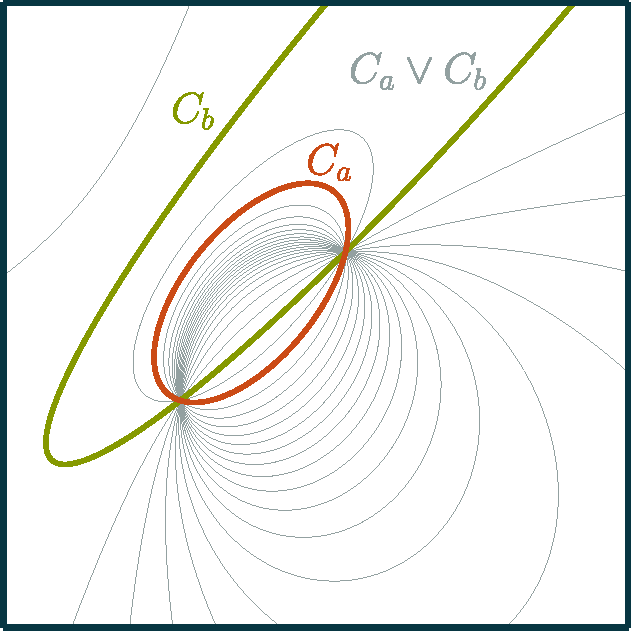
\includegraphics[width=\linewidth]{CaVeeCb}
        \subcaption{}\label{fig:constraints:a}
    \end{subfigure}
    \begin{subfigure}[t]{0.32\textwidth}
        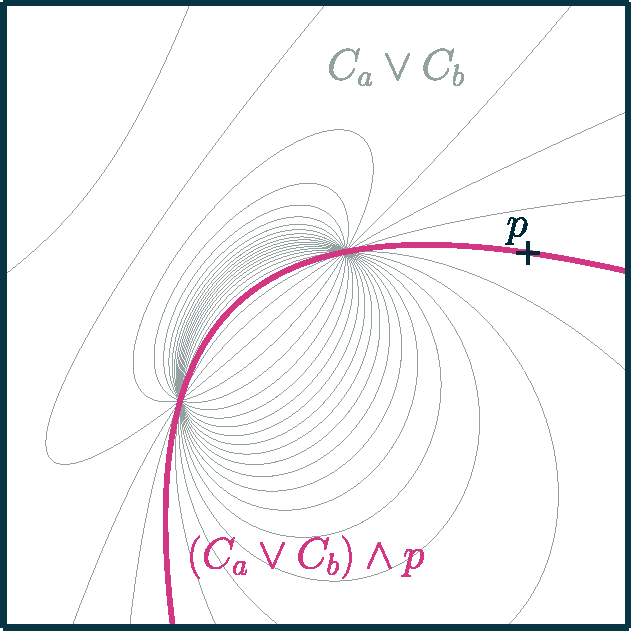
\includegraphics[width=\linewidth]{CaVeeCbWedgep}
        \subcaption{}\label{fig:constraints:b}
    \end{subfigure}
    \begin{subfigure}[t]{0.32\textwidth}
        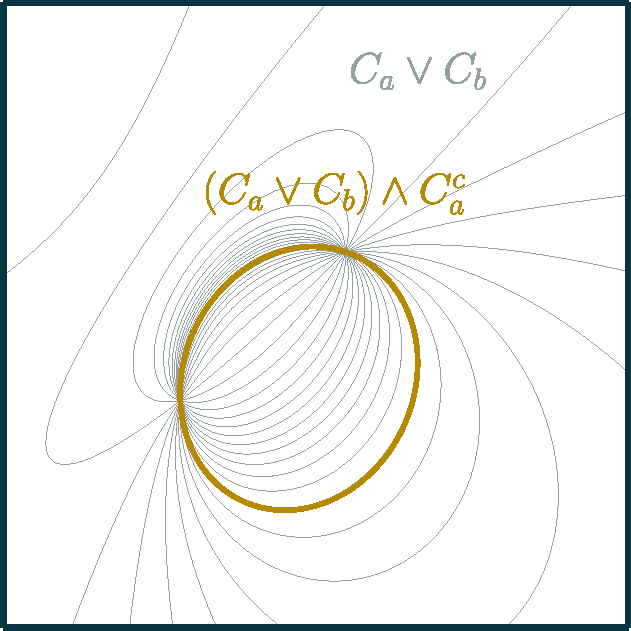
\includegraphics[width=\linewidth]{CaVeeCbWedgeCac}
        \subcaption{}\label{fig:constraints:c} 
    \end{subfigure}
    \captionsetup{subrefformat=parens}
    \caption{In~\subref{fig:constraints:a} a \(2\)-pencil is generated by two conics \(C_a\) and \(C_b\). This same pencil is then constrained in~\subref{fig:constraints:b} by a point and in~\subref{fig:constraints:c} by the right complement of one of its conics. These figures respectively illustrate Th.~\ref{th:constraint-add-conic}, \ref{th:constraint-add-point} and~\ref{th:constraint-remove-conic}.}
    \label{fig:constraints}
\end{figure}


\begin{theorem}\label{th:constraint-remove-point}
    Consider \(P\) a pencil and \(\mathrm{p}\) a \(1\)-PSE in \(P\).
    \(P\vee \mathrm{p}^c\) is the pencil~\(P\) extended with the conic \(\mathrm{p}^c\), which means that \(P\vee \mathrm{p}^c\) is the pencil \(P\) without the constraint of the \(1\)-PSE \(\mathrm{p}\).
\end{theorem}
\begin{proof}
    Let \(P\) be a pencil containing a \(1\)-PSE \(\mathrm{p}\). Let \(P'\) be a sub-pencil of \(P\) so that \(P = P'\wedge \mathrm{p}\).
    \begin{equation}
    P \vee \mathrm{p}^c = (P' \wedge \mathrm{p}) \vee \mathrm{p}^c \equiv P'
    \end{equation}
\end{proof}
These theorems allow to consider, construct, and manipulate every geometric object of QC2GA as either pencils or PSE. Table~\ref{tab:objets-as-pencils-or-pse} displays the correspondence of QC2GA's object and PSE and pencils.

\begin{table}[!ht]
    \centering
\setlength{\tabcolsep}{3ex}
    \begin{tabular}{l|c}
       Point  &  real \(1\)-PSE\\
       tuple of \(n\) points & real \(n\)-PSE \\
       tuple of infinite points and improper objects & \(n\)-PSE \\
       conic & \(1\)-pencil \\
       intersection of \(n\) conics & \(n\)-pencil
    \end{tabular}
    \caption{QC2GA objects as PSEs or pencils.}
    \label{tab:objets-as-pencils-or-pse}
\end{table}

\subsection{Real and Imaginary pencils and intersections}

Pencils have been introduced in a general way as objects constructed from any PSEs. This section introduces the concept of real and imaginary pencils and their application to the sum of conics.
\begin{definition}[Real Pencil]
    A real pencil \(P\) is a pencil of the form \(P = I_o^\triangleright\wedge\mathrm{p}\) with \(\mathrm{p}\in \mathrm{RePSE}\).
\end{definition}
% \begin{definition}[Imaginary Pencil]
%     A real pencil \(P\) is a pencil of the form \(P = I_o^\triangleright\wedge\mathrm{p}\) with \(\mathrm{p}\in \mathrm{RePSE}\).
% \end{definition}
\begin{definition}[Imaginary Pencil]
    An imaginary pencil \(P\) is a pencil of the form \(P = I_o^\triangleright\wedge\mathrm{p}\) with \(\mathrm{p}\in \mathrm{ImPSE}\).
\end{definition}
Consider \(k\) conics \(C_1,\dots,C_k\) intersecting the real \(n\)-PSE
\(\mathrm{p}^n_{Int}\in \mathrm{RePSE}_n\). They all can be factored into the real pencil \(I_o^\triangleright\wedge \mathrm{p}^n_{Int}\) and a \((5-n)\)-PSE \(r_i\) \(\forall i\in[1,k])\) containing the remainder of the conics' information. Doing so allows factoring any linear sum of these conics.
\begin{align}\label{eq:k-conics-to-intersect}
    \forall i \in [1,k], C_i &= I_o^\triangleright \wedge \mathrm{p}^n_{Int} \wedge r_i \\
    \sum_{i=1}^k \lambda_i C_i &= I^\triangleright_o \wedge \mathrm{p}^n_{Int} \wedge \sum_{i=1}^k \lambda_i r_i  \\
    \bigvee_{i=1}^k  C_i &= I^\triangleright_o \wedge \mathrm{p}^n_{Int} \wedge R  
\end{align}
The real pencil \(I_o^\triangleright \wedge \mathrm{p}_{Int}^n\) is by Th.~\ref{th:constraint-add-point} the set of all conics passing through the real \(n\)-PSE of intersection points \(\mathrm{p}_{Int}^n\). The remaining terms \(r_i\) determine the imaginary PSE \(R\) of the intersection in the complementary space of the real pencil. 
\begin{align}
    \forall i \in [1,k], r_i &= C_i \vee \left(I_o^\triangleright \wedge \mathrm{p}_{Int}^n\right)^c \\
    R &= \left(\bigvee_{i=1}^k C_i\right) \vee \left(I_o^\triangleright\wedge \mathrm{p}_{Int}^n\right)^c
\end{align}
\(R\) is the "intersection of \(r_1,\dots,r_k\) in the subspace \(\left(I_o^\triangleright \wedge \mathrm{p}^n_{Int}\right)^c\)"; it is not possible to just intersect the residuals \(r_i\) to compute \(R\). This imaginary PSE has the sole effect of doing a projection in the real pencil while keeping the number of intersection points constant. This leads to the following theorem:

\begin{theorem}
    The pencil \(P\) generated by \(n\in[0,6]\) linearly independent conics \(C_1,\dots,C_{n}\) intersecting on \(k\in[0,6-n]\) common points \(\mathrm{p}^k\) is of the form:
    \begin{align}
        P &= \bigvee_{i=1}^{6-n} C_i = I_o^\triangleright \wedge \mathrm{p}^k\wedge r & (\mathrm{p}^k,r)\in \mathrm{RePSE}_k\times\mathrm{ImPSE}_{6-n-k}     
    \end{align}
\end{theorem}
\begin{proof}
    The conics in \(P\) pass through the points of the real \(k\)-PSE \(\mathrm{p}^k\) therefore it is of the form \(I_o^\triangleright \wedge \mathrm{p}^k \wedge r\) with~\(r\) the remainder of the blade $\big($a~\((6-n-k)\)-PSE $\big)$. Since all the intersection points are \(\mathrm{p}^k\), then there are no points in~\(r\), therefore~\(r\) is an imaginary PSE.
\end{proof}

\begin{definition}[\(n\)-intersection]
A \(n\)-intersection is a pencil containing \(n\) points.
\end{definition}

\begin{remark}
The imaginary pencils are the \(0\)-intersections.
\end{remark}
\begin{remark}
\(n\)-intersections are \(k\)-pencils with \(k \ge 6-n\).
\end{remark}
\noindent The introduction of pencils and intersections concludes with this section. An illustrative case will be detailed in Sec.~\ref{sec:example-3-pencil}.



\subsection{Example of a pencil of three conics}
\label{sec:example-3-pencil}
This section, illustrated by Fig.~\ref{fig:pencil-3}, aims to provide an example of the proposed results on a pencil more complex than a \(2\)-pencil. A \(3\)-pencil (or \(3\)-intersection) is created from points, then an orthogonal basis is extracted from this pencil, and the \(3\)-pencil is constrained into two different \(2\)-pencils.


\begin{figure}
    \centering
    \begin{subfigure}[t]{0.32\textwidth}
        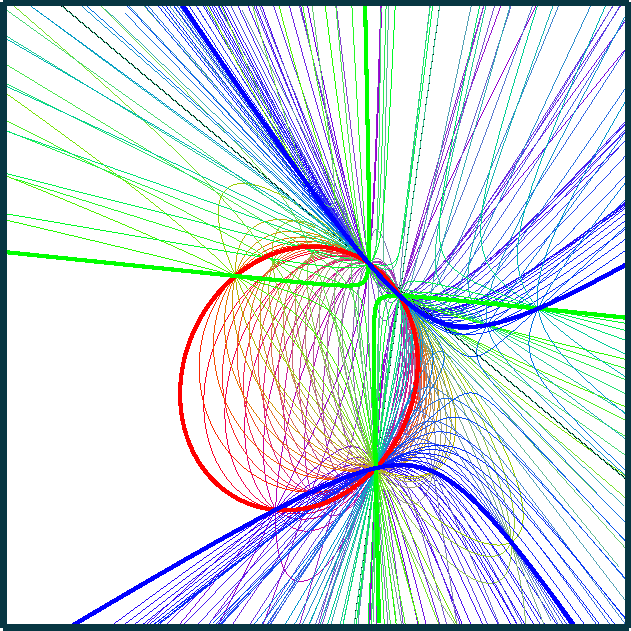
\includegraphics[width=\textwidth]{pencil-onion}
        \subcaption{}\label{fig:pencil-3:rgb} 
    \end{subfigure}
    \begin{subfigure}[t]{0.32\textwidth}
        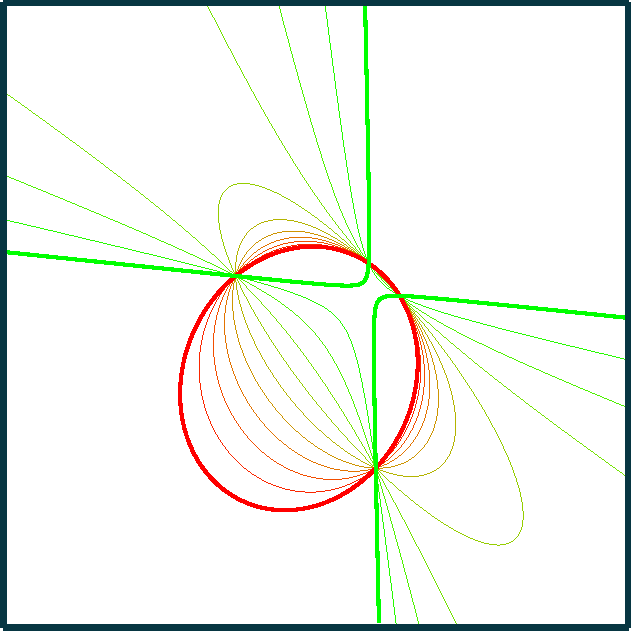
\includegraphics[width=\textwidth]{pencil-onion-12}
    \subcaption{}\label{fig:pencil-3:rg} 
    \end{subfigure}
    \begin{subfigure}[t]{0.32\textwidth}
        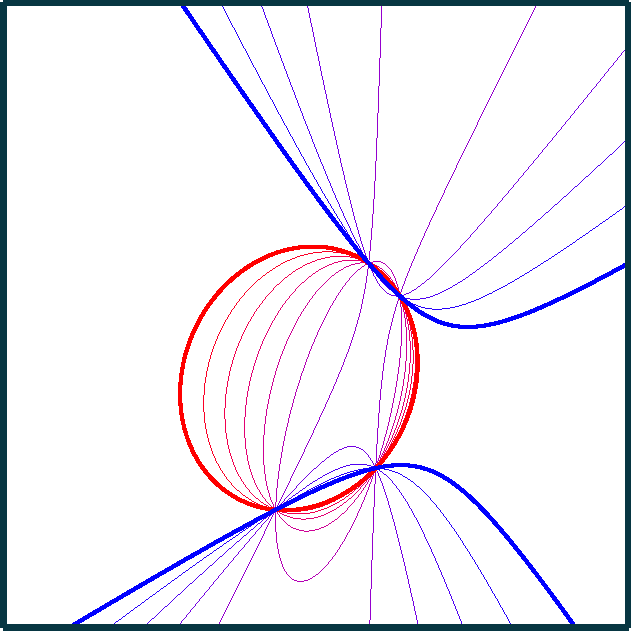
\includegraphics[width=\textwidth]{pencil-onion-13}
        \subcaption{}\label{fig:pencil-3:rb} 
    \end{subfigure}
    \captionsetup{subrefformat=parens}
    \caption{A pencil generated by three points (or by three conics sharing three common points) and two sub-pencils generated by four points. The color represents the coordinate of the conics within the 3-pencil, with each primary color associated with a conic of one of its orthogonal basis.}
    \label{fig:pencil-3}
\end{figure}
\noindent Fig.~\ref{fig:pencil-3:rgb} is built by generating six points \(\mathrm{p}_1, \dots, \mathrm{p}_6\). These points are the generators of the minimal pencil \(P = \mathrm{p}_1 \wedge \mathrm{p}_2 \wedge \mathrm{p}_3 \wedge I_o^\triangleright\) and then three orthogonal conics (see Def.~\ref{def:orthogonalconics})
\begin{align}
    C_r &= P \wedge \mathrm{p}_4 \wedge \mathrm{p}_5 \\
    C_g &= P \wedge C_r^c \wedge \mathrm{p}_6 \\
    C_b &= P \wedge C_r^c \wedge C_g^c 
\end{align}
These conics are enough to span the whole pencil \(P\). The two other pencils of Fig.~\ref{fig:pencil-3:rg} and~\ref{fig:pencil-3:rb} are just the pencils generated by \((C_r, C_g)\) and \((C_r, C_b)\), which are also \(P\) constrained by \(C_b\) and \(C_g\).
\begin{align}
    P~~&= C_r \vee C_g \vee C_b \\
    P_{rg} &= C_r \vee C_g = P \wedge C_b^c\\
    P_{rb} &= C_r \vee C_b = P \wedge C_g^c
\end{align}
Every conic of \(P\) meets in \(\mathrm{p}_1, \mathrm{p}_2, \mathrm{p}_3\), but the two other intersection points in \(P_{rg}\) and \(P_{rb}\) are not \(\mathrm{p}_4, \mathrm{p}_5, \mathrm{p}_6\). This is because we did not specifically chose a slice of \(P\) in which these points are intersection points of the pencil. Such sub-pencils would be \(P\wedge \mathrm{p_4}\), \(P\wedge \mathrm{p_5}\) and \(P\wedge \mathrm{p_6}\).
%%%%%%%%%%%%%%%%%%%%%%%%%%%%%%%%%%%%%%%%%%%%%%%%%%%%%%%%%%%%%%%%%%%%%%%%%%%%%%%%%%%%%%%%%%%%%%%%%%%%%%%%%%%%%
%%%%%%%%%%%%%%%%%%%%%%%%%%%%%%%%%%%%%%%%%%%%%%%%%%%%%%%%%%%%%%%%%%%%%%%%%%%%%%%%%%%%%%%%%%%%%%%%%%%%%%%%%%%%%
\section{Computing discriminants in QC2GA}
\label{sec:discriminants}
The anti-outer product can be used to compute the discriminants \(\Delta_2, \Delta_3\) of Eq.~\eqref{eq:discriminants} and even the center point \(\mathrm{p}_c\) of a conic.

\begin{proposition}
    Consider a conic \(C\) of parameters \((a,b,c,d,e,f)\).
    The discriminant of \(C\) and its center point can be computed using three lines:
    \begin{align}
    l_1 &= \left(a e_1 + \frac{c}{2} e_2 - \frac{d}{2} e_\infty\right)^* \\
    l_2 &= \left(\frac{c}{2} e_1 + b e_2 - \frac{e}{2} e_\infty\right)^* \\
    l_3 &= \left(\frac{d}{2} e_1 + \frac{e}{2} e_2 - f e_\infty\right)^* \\
    l_1 \vee l_2 &= -\frac{1}{2}\left(\underbrace{w_c}_{\Delta_2} e_o + x_c e_{1} + y_c e_{2}\right) \wedge I_o^\triangleright \wedge I_\infty  \equiv \mathrm{p}_c \wedge I_o^\triangleright \wedge I_\infty  \\
    l_1 \vee l_2 \vee l_3 &= \frac{1}{2}\Delta_3 I_o^\triangleright\wedge I_\infty
    \end{align}
    The coordinates of \(l_1\vee l_2\) are the projective coordinates \(x_c, y_c, w_c\) of the point of the center of the conic \(\mathrm{p}_c\). This pencil is a flat point as introduced by~\cite{breuils_three-dimensional_2019} and finds geometric interpretation.% The homogeneous coordinate \(w_c\) is equal to the determinant \(\Delta_2\) , which makes sense since when this term is 0, the center point lies at infinity since the conic is a parabola.
\end{proposition}

\begin{proof}
\begin{align}
&l_1 \vee l_2 = 
-\frac{1}{2}\left( \underbrace{(ab-\frac{c^2}{4})}_{\Delta_2, w_c} e_o + \underbrace{(\frac{ce}{4}-\frac{bd}{2})}_{x_c} e_{1} + \underbrace{(\frac{cd}{4}-\frac{ae}{2})}_{y_c}  e_{2}\right) \wedge I_o^\triangleright \wedge I_\infty  \\
& l_1\vee l_2\vee l_3= \frac{1}{2}\underbrace{\left(abf+\frac{cde-c^2f-bd^2-ae^2}{4}\right)}_{\Delta_3} I_o^\triangleright\wedge I_\infty
\end{align}
\end{proof}

\noindent This enables us to enhance already existing algorithms with Geometric Algebra by using the wedge product to compute the discriminants and center of the conic.

\section{Extracting points from an intersection}
\label{sec:extraction}
Let \(Inter\) be the intersection of two unknown conics. Sec.~\ref{sec:pencils} introduces the fact that this object is a pencil generated by four \(1\)-PSEs. The next objective is to extract the points contained in this pencil. 

The approach followed in this paper consists in first finding a degenerate conic \(C_{deg}\) in \(Inter\) and another conic \(C_{other}\) orthogonal to \(C_{deg}\). Then, this degenerate conic is split into two lines. The conic intersection problem becomes a line-to-conic intersection, which is easier to solve.



\paragraph{\textbf{Finding a degenerate conic (Algorithm~\ref{alg:find_degen})}}
A random conic \(C_a\) and its orthogonal conic \(C_b\) are first sampled in \(Inter\) by using a random point \(\mathrm{p}\).
\begin{align}
C_a &= Inter \wedge \mathrm{p} \\
C_b &= Inter \wedge C_a^c
\end{align}
Then, find \(\lambda\) and \(\mu\) in \(\mathbb{R}\) so that \(\Delta_3(\lambda C_a + \mu C_b) = 0\). This is achieved using the following general formula, based on the definition of \(\Delta_3\) in Sec.~\ref{sec:discriminants}:
\begin{align}
\forall i \in [1,6], E_i &= \mathcal{B}_{p}[i]\\
\Gamma(i,j,k) &= \Delta_3(Inter\wedge(E_i + E_j + E_k)) - \Delta_3(Inter\wedge(E_i + E_j)) \notag\\ &- \Delta_3(Inter\wedge(E_i + E_k)) - \Delta_3(Inter\wedge(E_j + E_k)) \notag\\
&+ \Delta_3(Inter\wedge E_i) + \Delta_3(Inter\wedge E_j) + \Delta_3(Inter\wedge E_k)  \\
\Delta_3(C) &= \frac{1}{6} \sum_{i,j,k\in[1,6]} \Gamma_3(i,j,k) x_i x_j x_k
\end{align}
Here the terms \(\Gamma(i,j,k)\) are only there for the sake of clarity.
In that particular case, the formula results in:
\begin{align}
    \Delta_3(\lambda C_a + \mu C_b) &= \Delta_3(C_a)\lambda^3 + \Delta_3(C_b)\mu^3 \\
    &+ \left(\frac{\Delta_3(C_a+C_b) - \Delta_3(C_a - C_b)}{2}-\Delta_3(C_b)\right) \lambda^2\mu \\&+ \left(\frac{\Delta_3(C_a+C_b)  + \Delta_3(C_a - C_b)}{2}-\Delta_3(C_a)\right) \lambda\mu^2 
\end{align}
The root of that cubic polynomial is found using:
\begin{align}
\span u_1x^3+u_2x^2+u_3x+u_4=0\\
\Delta_0 &= u_2^2 - 3u_1u_3 &
\Delta_1 &= 2u_2^3 - 9u_1u_2u_3 + 27u_1^2u_4 \\
\Omega_{\pm} &= \sqrt[3]{\frac{\Delta_1 \pm \sqrt{\Delta_1^2 - 4\Delta_0^3}}{2}}
&x_k &= -\frac{u_2 + e^{i\frac{2\pi k}{3}}\Omega_{+} + e^{i\frac{-2\pi k}{3}}\Omega_{-}}{3u_1} &
\end{align}
with \(x_0\) being always real.
The above formulas are the base of Algorithm~\ref{alg:find_degen}.

\begin{center}
\begin{algorithm}[t] \SetAlgoLined
\Fn{\funct{gen\_degen\_and\_other}}{  % \func: see macro at usepackage 
\KwIn{\(Inter\)}
\KwOut{\(C_{deg}, C_{\bot}\)}
\BlankLine
\lDo{\(\mathrm{p}_a\wedge \mbox{Inter} = 0\)}{\(\displaystyle \mathrm{p}_a \leftarrow  \mbox{random\_point}()\)}

\(\displaystyle C_a \leftarrow  Inter \wedge \mathrm{p}_a  
\qquad C_b \leftarrow Inter \wedge (C_a^{c})\)\;
\(\displaystyle a\leftarrow\Delta_3(C_b) \qquad b \leftarrow \frac{\Delta_3(C_a+C_b) + \Delta_3(C_a-C_b)}{2} - \Delta_3(C_a)\)\;
\(\displaystyle d \leftarrow \Delta_3(C_a) \qquad c \leftarrow \frac{\Delta_3(C_a+C_b) - \Delta_3(C_a-C_b)}{2} - \Delta_3(C_b)\)\;
\(\displaystyle \Delta_0 \leftarrow b^2 - 3ac  \qquad
 \Delta_1 \leftarrow 2b^3 - 9abc + 27a^2d\)\;
\(\displaystyle \Omega_{-} \leftarrow \sqrt[3]{\frac{\Delta_1 - \sqrt{\Delta_1^2 - 4\Delta_0^3}}{2}}\) \qquad \(\displaystyle \Omega_{+} \leftarrow \sqrt[3]{\frac{\Delta_1 + \sqrt{\Delta_1^2 - 4\Delta_0^3}}{2}}\)\;
\(\displaystyle \lambda \leftarrow -3a\)\qquad
\(\displaystyle \mu \leftarrow b + \Omega_{-} + \Omega_{+}\)\;
\(\displaystyle C_{deg} \leftarrow \lambda C_a + \mu C_b \qquad C_{\bot} \leftarrow -\mu C_a + \lambda C_b\)\;
\caption{Find a degenerate conic and a different one in the pencil of \(Inter\)}
\label{alg:find_degen}
}
\end{algorithm}
\end{center}
\paragraph{\textbf{Factorize pair of lines (Algorithm \ref{alg:factor_pair})}}

A pair of lines is of the form:
\begin{align}
l_1 &= \cos(\alpha_1) x + \sin(\alpha_1) y + w_1 \\
l_2 &= \cos(\alpha_2) x + \sin(\alpha_2) y + w_2 \\
C &: \nu l_1  l_2 = ax^2 + by^2 + cxy + dx + ey + f = 0
\end{align}
with \(\nu \in \mathbb{R}^*\) a multiplicative constant coming from the projective aspect of the conic. These two lines can be extracted using the method presented by Richter-Gebert~\cite{richter-gebert_perspectives_2011}. This method is also used by Byrtus et al.~\cite{byrtus_specific_2021} for their specific GAC intersection extraction.
\begin{center}
\begin{algorithm}[H]
\SetAlgoLined
\Fn{ \funct{factor\_line\_pair}}{  
\KwIn{\(C_{deg}\)}
\KwOut{\(\alpha_1, \alpha_2, w_1, w_2\) \tcp*{lines angles and offsets}} 
\BlankLine
\(\displaystyle H \leftarrow \mbox{hessian\_matrix}(C_{deg})\)\quad \(A \leftarrow \mbox{adj}(H)\) \quad \(\displaystyle i \leftarrow \mbox{argmin}_k\{A_{k,k}\}\) \\
\(\displaystyle D \leftarrow \begin{bmatrix}
    0                  & -A_{i,2} & +A_{i,1} \\
    +A_{i,2} & 0                  & -A_{i,0} \\
    -A_{i,1} & +A_{i,0} & 0 
\end{bmatrix}/\sqrt{-A_{i,i}}\) \quad \(\displaystyle N \leftarrow H + D\)\;
\(\displaystyle u_1,v_1,w_1 \leftarrow N\Big[*, \mbox{argmax}_j\{N[1,j]^2 + N[2,j]^2]\}\Big]\)\\
\(\displaystyle u_2,v_2,w_2 \leftarrow N\Big[\mbox{argmax}_j\{N[j,1]^2 + N[j,2]^2]\}, *\Big]\)\\
\(\alpha_1 \leftarrow \mbox{arctan2}(v_1, u_1)  \quad \alpha_2 \leftarrow \mbox{arctan2}(v_2,u_2)\)\;
\Return \(\{\alpha_1, \alpha_2, w_1/\sqrt{u_1^2 + v_1^2}, w_2/\sqrt{u_2^2 + v_2^2}\}\) 
\caption{Pair of lines factorization algorithm}
\label{alg:factor_pair}
}
\end{algorithm}
\end{center}

\paragraph{\textbf{Conic-line intersection (Algorithm \ref{alg:conic_line_inter})}}
The idea is to rotate the system so that the line is aligned with the \(y\) axis (which means a known $x$). The system results in  a trivial quadratic polynomial in $y$.


\begin{center}
\begin{algorithm}[H]
\SetAlgoLined
\Fn{ \funct{conic\_line\_inter}}{  % \func: see macro at usepackage 
\KwIn{\(C,\theta, w\)}
\KwOut{points}
\BlankLine
\(R \leftarrow \mbox{qc2ga\_rotor}(-\theta)\)\quad\(\displaystyle [a,b,c,d,e,f] \leftarrow R C \tilde R\)\;
\(\displaystyle x \leftarrow - w \) \qquad
\(\displaystyle \delta \leftarrow (cx + e)^2 - 4b(ax^2 + dx + f) \qquad \gamma \leftarrow  \frac{cx + e}{2b}\)\;
\(\displaystyle  \mathrm{p}_0 \leftarrow \begin{pmatrix}\cos(\theta)x - \gamma \sin(\theta) \\ \sin(\theta)x + \gamma \cos(\theta)\end{pmatrix} \qquad \vec{u} \leftarrow \frac{1}{2b}\begin{pmatrix}-\sin(\theta)\\ \cos(\theta)\end{pmatrix}\)\;
\Switch{\mbox{sgn}(\(\delta\))}
{
    \lCase{\(+\)}{\Return\{\(\mathrm{p}_0 \pm \sqrt{\delta}\vec{u}\)\}}
    \lCase{\(\,0\,\)}{\Return \{\(\mathrm{p}_0\)\}}
    \lCase{\(-\)}{\Return\{\}}
}
\caption{Conic-Line intersection algorithm}
\label{alg:conic_line_inter}
}
\end{algorithm}
\end{center}


\subsection{Full algorithm}

The full algorithm to compute conics intersection points is just the succession of the three algorithms described in the previous section, as presented in Algorithm \ref{alg:pts_extract}.
%Using the algorithms we just presented, we can write the algorithm \ref{alg:pts_extract} that extracts the real points in an intersection object.
\begin{center}
\begin{algorithm}[H]
\SetAlgoLined
\Fn{ \funct{extract\_pts\_from\_inter}}{  % \func: see macro at usepackage 
\KwIn{\(Inter\)}
\KwOut{a set of points}
\BlankLine
\(C_{deg}, C_{\bot} \leftarrow\) gen\_degen\_and\_other(\(Inter\))\;
\(\alpha_1,\alpha_2,w_1,w_2 \leftarrow\) factor\_line\_pair(\(C_{deg}\))\;
\Return~conic\_line\_inter(\(C_{\bot},\alpha_1, w_1\))~\(\cup\)~conic\_line\_inter(\(C_{\bot},\alpha_2, w_2\))\;
\caption{Point extraction algorithm}
\label{alg:pts_extract}
}
\end{algorithm}
\end{center}



%%%%%%%%%%%%%%%%%%%%%%%%%%%%%%%%%%%%%%%%%%%%%%%%%%%%%%%%%%%%%%%%%%%%%%%%%%%%%%%%%%%%%%%%%%%%%%%%%%%%%%%%%%%%%
%%%%%%%%%%%%%%%%%%%%%%%%%%%%%%%%%%%%%%%%%%%%%%%%%%%%%%%%%%%%%%%%%%%%%%%%%%%%%%%%%%%%%%%%%%%%%%%%%%%%%%%%%%%%%
%%%%%%%%%%%%%%%%%%%%%%%%%%%%%%%%%%%%%%%%%%%%%%%%%%%%%%%%%%%%%%%%%%%%%%%%%%%%%%%%%%%%%%%%%%%%%%%%%%%%%%%%%%%%%
%%%%%%%%%%%%%%%%%%%%%%%%%%%%%%%%%%%%%%%%%%%%%%%%%%%%%%%%%%%%%%%%%%%%%%%%%%%%%%%%%%%%%%%%%%%%%%%%%%%%%%%%%%%%%
%%%%%%%%%%%%%%%%%%%%%%%%%%%%%%%%%%%%%%%%%%%%%%%%%%%%%%%%%%%%%%%%%%%%%%%%%%%%%%%%%%%%%%%%%%%%%%%%%%%%%%%%%%%%%
%%%%%%%%%%%%%%%%%%%%%%%%%%%%%%%%%%%%%%%%%%%%%%%%%%%%%%%%%%%%%%%%%%%%%%%%%%%%%%%%%%%%%%%%%%%%%%%%%%%%%%%%%%%%%
\section{Numerical experiments}
\label{sec:experiments}

The proposed method has been implemented in C++ using Garamon~\cite{breuils_garamon_2019} with double floating point precision in the public repository \url{https://github.com/technolapin/qc2ga-intersection}.Fig.~\ref{fig:2} shows a few examples computed with our code from QC2GA intersection objects.

\begin{figure}
    \begin{center}
    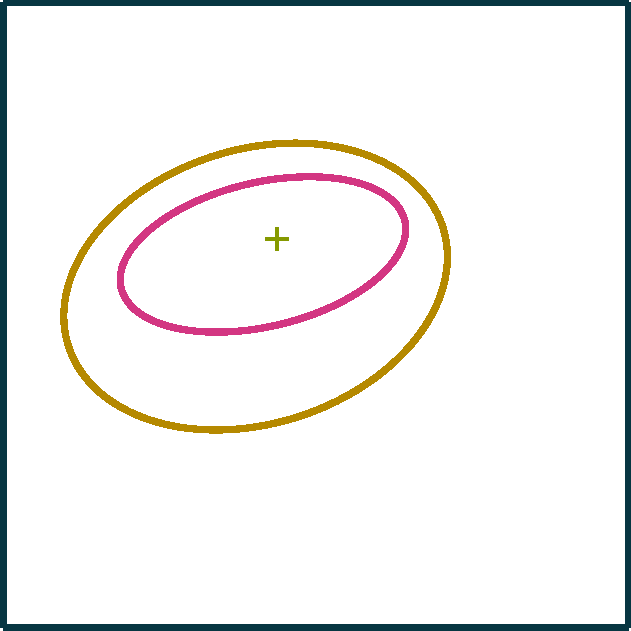
\includegraphics[width=0.35\linewidth]{0-inter-59912347}
    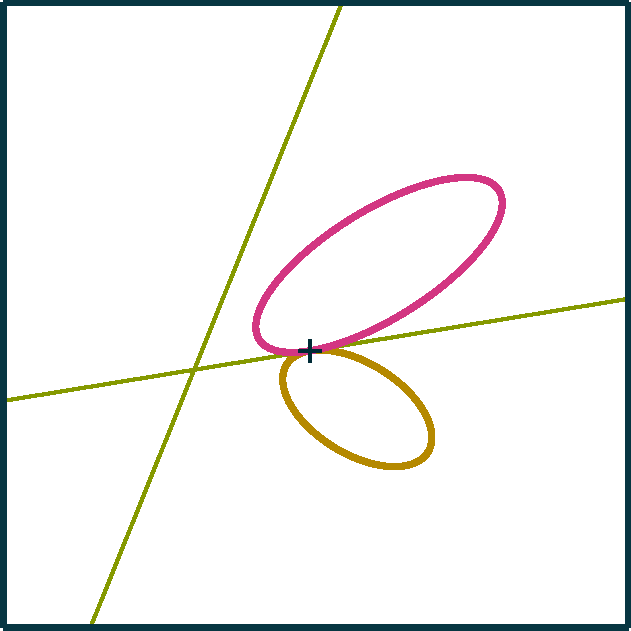
\includegraphics[width=0.35\linewidth]{1-inter-21321560}
    
    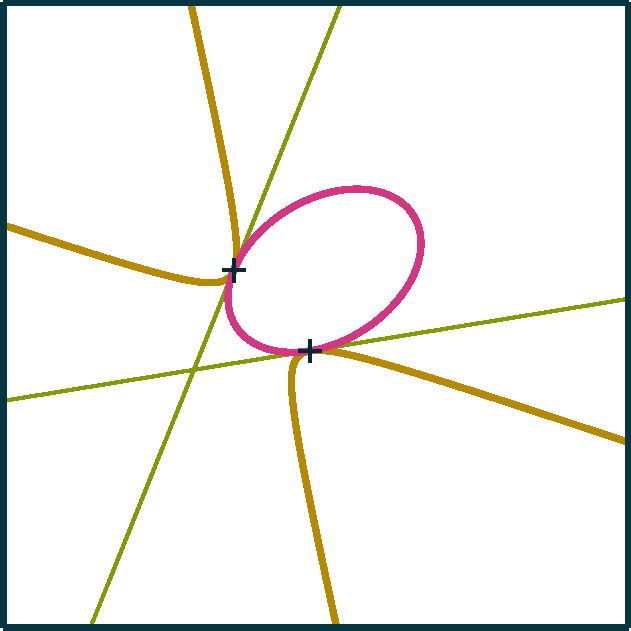
\includegraphics[width=0.35\linewidth]{2-inter-21321560}
    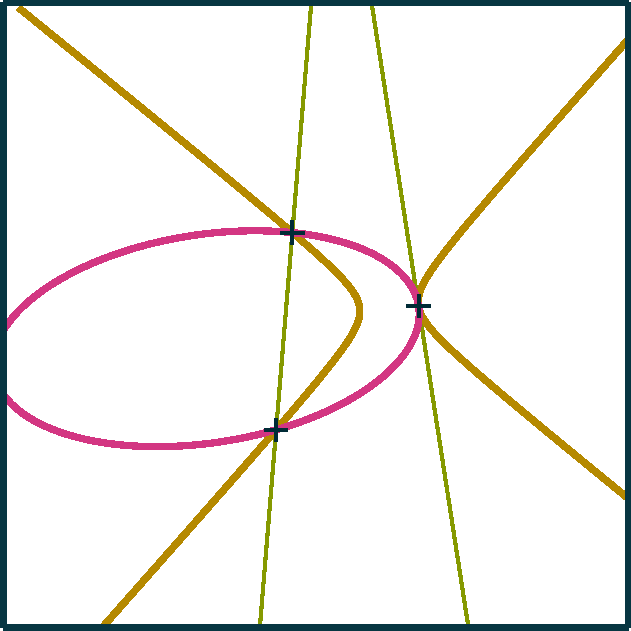
\includegraphics[width=0.35\linewidth]{3-inter-59912348}
    
    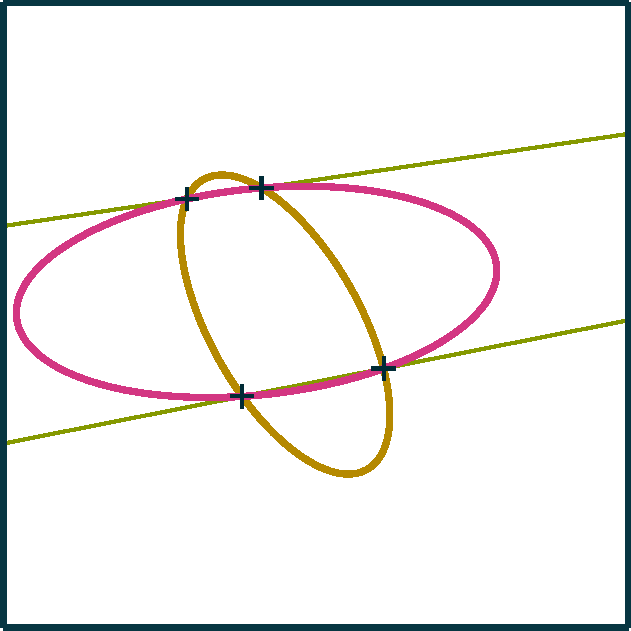
\includegraphics[width=0.35\linewidth]{4-inter-2132132572}
    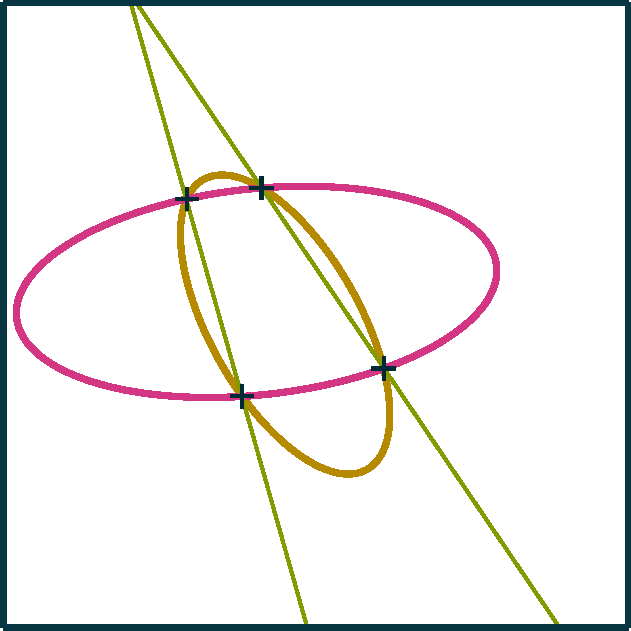
\includegraphics[width=0.35\linewidth]{4-inter-2132132572-alternative}
    \end{center}
 \caption{Extraction of 0,1,2,3 and 4-intersections where the green curve is the degenerate conic, which can be a pair of lines or a point. The 4-intersection is depicted twice with different pairs of lines.}	\label{fig:2}
\end{figure}



We conducted some tests to evaluate the numerical behavior of our implementation. These tests run on various random $n$-intersections.
In each case, some random points are generated with a uniform distribution in \([-1,1]^2\). Five of these points are used to build a conic. Then two lines are generated to build a degenerate conic. Those lines are chosen so that the pair of lines intersects the first conic at the desired number of points. The first conic and the degenerate one are then intersected, resulting in an intersection object of known type (0, 1, 2, 3 or 4-intersection).

Given this controlled data, we apply our method to extract the points of these intersection objects. These results are compared with the input data. As a testing metric, we first check whether the correct number of intersecting points has been successfully computed. An incorrect number of points is counted as a failure. Then, we also check the accuracy of the point extraction. For this purpose, each extracted point is compared to its corresponding point with a simple wedge product. This results in a scalar close to 0. Whenever that scalar is not close enough to 0 (more than a decided threshold set to 0.001), this is counted as an error as well.
This procedure of tests ran on 1,000,000 iterations, and the results are presented in Table~\ref{tab:results}.
\begin{table}[!ht]
    \begin{center}
    \begin{tabular}{l|c|c|c|c|c|c}
        kind of& success rate &\multicolumn{5}{c}{Errors are interpreted as}\\
        intersection& (\%)& 0-inter & 1-inter & 2-inter & 3-inter & 4-inter\\
        \hline
0-inters & 99.9997 & 0 &         0 & 0.0003 &          0 &          0 \\
1-inters & 99.5909 & 0 & 0.0638999 &  0.333 &      0.011 &     0.0012 \\
2-inters & 99.8390 & 0 & 0.0263999 & 0.1148 &  0.0179999 & 0.00179999 \\
3-inters & 99.9806 & 0 &    0.0017 & 0.0121 & 0.00389999 &     0.0017 \\
4-inters & 99.9889 & 0 &    0.0002 & 0.0003 &     0.0094 &     0.0012 
    \end{tabular}
    \end{center}
\caption{Success rate of the conic intersection computation method on 1,000,000 random 0,1,2,3 and 4-intersections. A failure corresponds to the case where the number of expected points found is incorrect or where the computed points do not lie on the intersection. The failures are classified according to the number of points found.}	\label{tab:results}
\end{table}
These tests encounter an "issue": some errors (like finding a wrong 0-intersection) are so unlikely to happen that none were found. A lack of such errors makes it hard to tell how likely these errors are, but this also suggests that the algorithm is very stable and robust.


\section{Conclusion}
\label{sec:conclusion}
This paper shows the equivalence of QC2GA and GAC and how this equivalence is profitable for both of them. A novel interpretation of QC2GA is also presented, based on pencils of conics built from point-space elements. 
This new way of thinking QC2GA's objects allows new set of operations, such as building and constraining pencils from conics and points by using their right-complement. This new toolbox permits the extraction of orthogonal conics from any intersection object, as well as computing the discriminants and center points of conics. These new capabilities allow the establishment of a new geometric-algebra-powered algorithm for extracting the intersection points of an intersection object of two conics.
This framework, based on pencils of conics and point-space elements, can be adapted to many other algebra and therefore could be used to manipulate many other curves and objects. A trivial example would be C2GA, since this algebra is embedded in QC2GA. It would be interesting in many situations to think in terms of pencils of curves, for the same reasons as those encountered in this paper.
This approach could also be of use outside the Geometric Algebra community, as some of the tools, such as finding two orthogonal conics from an \(2\)-pencil of conics, can easily be adapted to linear algebra and are useful in terms of numerical stability when trying to find the intersection points of two conics.

As a future work, we intend to work in CGA to demonstrate the pertinence of the pencil framework in that popular Geometric Algebra.


\bibliographystyle{spmpsci}
\bibliography{geometric-algebra}

\end{document}

